% Arquivo LaTeX de exemplo de dissertação/tese a ser apresentados à CPG do IME-USP
%
% Versão 6: Sex Nov  10 18:00:00 BRT 2017
%
% Criação: Jesús P. Mena-Chalco
% Revisão: Fabio Kon e Paulo Feofiloff
% Adaptação para UTF8, biblatex e outras melhorias: Nelson Lago


%%%%%%%%%%%%%%%%%%%%%%%%%%%%%%%%%%%%%%%%%%%%%%%%%%%%%%%%%%%%%%%%%%%%%%%%%%%%%%%%
%%%%%%%%%%%%%%%%%%%%%%%%%%%%%%% PREÂMBULO LaTeX %%%%%%%%%%%%%%%%%%%%%%%%%%%%%%%%
%%%%%%%%%%%%%%%%%%%%%%%%%%%%%%%%%%%%%%%%%%%%%%%%%%%%%%%%%%%%%%%%%%%%%%%%%%%%%%%%

% Este pacote gera avisos durante a compilação sobre comandos
% considerados obsoletos.
\RequirePackage[l2tabu, orthodox]{nag}

% "Book" tem capítulos (e partes, mas normalmente não usamos) e, se o documento
% é frente-e-verso, cada capítulo começa em uma página de numeração ímpar.
% Report é similar, mas cada capítulo começa em uma nova página, par ou ímpar.
% É possível mudar esse comportamento com a opção "openany". Observe que você
% pode adaptar este modelo para escrever artigos, mudando a classe do
% documento de "book" para "article" ou a classe de algum periódico específico.
%
% A opção frente-e-verso aqui significa, por exemplo, que as margens das páginas
% ímpares e pares são diferentes ou que números de página aparecem à direita
% ou à esquerda alternadamente. Nada impede que você crie um documento "só
% frente" e, ao imprimir, faça a impressão frente-e-verso.
%
% Aqui também definimos a língua padrão do documento e línguas adicionais. A
% classe em si não usa essa informação mas, passando as opções de língua aqui,
% elas são repassadas para todas as demais classes, e diversas classes mudam
% seu comportamento em função da língua (em especial, babel/polyglossia).
% A última língua da lista é a língua padrão do documento.
%\documentclass[12pt,twoside,brazil,english]{book}
\documentclass[12pt,twoside,english,brazil]{book}
%\documentclass[12pt,twoside,english,brazil]{article}

% tamanho da página e margens
\usepackage[a4paper]{geometry}
\geometry{
  % distância entre o início da página e o início do texto principal
  top=32mm,
  bottom=28mm,
  left=24mm,
  right=34mm,
  % Com geometry, esta medida não é tão relevante; basta garantir que ela
  % seja menor que "top" e que o texto do cabeçalho caiba nela.
  headheight=25.4mm,
  % distância entre o início do texto principal e a base do cabeçalho;
  % ou seja, o cabeçalho "invade" a margem superior nessa medida. Essa
  % é a medida que determina a posição do cabeçalho
  headsep=11mm,
  footskip=10mm,
  marginpar=20mm,
  marginparsep=5mm,
}

% Vários pacotes e opções de configuração genéricos; para personalizar o
% resultado, modifique este arquivo.
%%%%%%%%%%%%%%%%%%%%%%%%%%%%%%%%%%%%%%%%%%%%%%%%%%%%%%%%%%%%%%%%%%%%%%%%%%%%%%%%
%%%%%%%%%%%%%%%%%%%%%%% CONFIGURAÇÕES E PACOTES BÁSICOS %%%%%%%%%%%%%%%%%%%%%%%%
%%%%%%%%%%%%%%%%%%%%%%%%%%%%%%%%%%%%%%%%%%%%%%%%%%%%%%%%%%%%%%%%%%%%%%%%%%%%%%%%

% Vários comandos auxiliares para o desenvolvimento de packages e classes;
% aqui, usamos em alguns comandos de formatação e condicionais.
\usepackage{etoolbox}
\usepackage{xstring}

% Detecta o tipo de sistema que estamos usando (XeTeX, LuaTeX ou pdfTeX). Na
% verdade, ifpdf não detecta pdfTeX, mas sim se estamos gerando um PDF; como
% só XeTeX, LuaTeX e pdfTeX geram PDFs, combinando todos é possível identificar
% pdfTeX também.
\usepackage{ifxetex}
\usepackage{ifluatex}
\usepackage{ifpdf}

% "fontenc" é um parâmetro interno do LaTeX. O fontenc default é OT1, mas ele
% tem algumas limitações; a mais importante é que, com ele, palavras acentuadas
% não podem ser hifenizadas. Por conta disso, quase todos os documentos LaTeX
% utilizam o fontenc T1. A escolha do fontenc tem consequências para as fontes
% que podem ser usadas no documento; hoje em dia T1 tem mais opções de
% qualidade, então não se perde nada.
\usepackage[T1]{fontenc}

% apenas útil para LaTeX tradicional e pdfTeX; XeTeX e LuaTeX usam sempre utf8.
\usepackage[utf8]{inputenc}

% Permite criar "headed lists", ou seja, "listas" de elementos que vão
% aparecendo ao longo do documento (como, por exemplo, teoremas). Podem ser
% também citações a autores específicos, seções de um documento que está
% sendo analisado etc. Precisa ser carregado antes das definições de fontes.
\usepackage{amsthm}

% Internacionalização dos nomes das seções ("chapter" X "capítulo" etc.),
% hifenização e outras convenções tipográficas. babel deve ser um dos
% primeiros pacotes carregados. É possível passar a língua do documento
% como parâmetro aqui, mas já fizemos isso ao carregar a classe, no início
% do documento.
\usepackage{babel}

% Comandos rápidos para mudar de língua:
% \en -> muda para o inglês
% \br -> muda para o português
% \texten{blah} -> o texto "blah" é em inglês
% \textbr{blah} -> o texto "blah" é em português
\babeltags{br = brazil, en = english}

% É possível personalizar as palavras-chave que babel utiliza, por exemplo:
%\addto\extrasbrazil{\renewcommand{\chaptername}{Chap.}}
% Com BibTeX, isso vale também para a bibliografia; com BibLaTeX, é melhor
% usar o comando "DefineBibliographyStrings".

% Para línguas baseadas no alfabeto latino, como o inglês e o português,
% o pacote babel funciona muito bem, mas com outros alfabetos ele às vezes
% falha. Por conta disso, o pacote polyglossia foi criado para substituí-lo.
% polyglossia só funciona com LuaTeX e XeTeX; como babel também funciona com
% esses sistemas, provavelmente não há razão para usar polyglossia, mas é
% possível que no futuro esse pacote se torne o padrão.
%\usepackage{polyglossia}
%\setdefaultlanguage{brazil}
%\setotherlanguage{english}

% microajustes no tamanho das letras, espaçamento etc. para melhorar
% a qualidade visual do resultado. LaTeX tradicional não dá suporte a
% nenhum tipo de microajuste; pdfLaTeX dá suporte a todos. LuaLaTeX
% e XeLaTeX dão suporte a alguns:
%
% * expansion não funciona com XeLaTeX
% * tracking não funciona com XeLaTeX; é possível obter o mesmo resultado
%   com a opção "LetterSpace" do pacote fontspec, mas a configuração é
%   totalmente manual. Por padrão, aumenta o afastamento entre caracteres
%   nas fontes "small caps"; o resultado não se presta ao uso na
%   bibliografia ou citações, então melhor desabilitar.
% * kerning e spacing só funcionam com pdfLaTex; ambas são funções
%   consideradas experimentais e nem sempre produzem resultados vantajosos.

\newcommand\microtypeopts{
  protrusion=true,
  tracking=false,
  kerning=false,
  spacing=false
}

\ifxetex
  \usepackage[expansion=false,\microtypeopts]{microtype}
\else
  \usepackage[expansion=true,\microtypeopts]{microtype}
\fi

% Alguns "truques" (sujos?) para minimizar over/underfull boxes.
%
% Para fazer um texto justificado, é preciso modificar o tamanho dos espaços
% em cada linha para mais ou para menos em relação ao seu tamanho ideal. Para
% escolher as quebras de linha, TeX vai percorrendo o texto procurando lugares
% possíveis para quebrar as linhas considerando essa flexibilidade mas dentro
% de um certo limite mínimo/máximo. Nesse processo, ele associa a cada possível
% linha o valor badness, que é o nível de distorção do tamanho dos espaços
% daquela linha em relação ao ideal, e ignora opções que tenham badness muito
% grande (esse limite é dado por \tolerance). Depois de encontradas todas as
% possíveis quebras de linha e a badness de cada uma, TeX calcula as penalties
% e demerits de cada possibilidade e escolhe a solução que minimiza o demerit
% total do parágrafo.
%
% Para cada fonte, o espaço em TeX tem um tamanho ideal, um tamanho mínimo e um
% tamanho máximo. TeX nunca reduz um espaço para menos que o mínimo da fonte,
% mas pode aumentá-lo para mais que o máximo. Se os espaços de uma linha ficam
% com o tamanho ideal, a badness da linha é 0; se o tamanho é
% reduzido/aumentado 50% do mínimo/máximo, a badness da linha é 12; se o
% tamanho é reduzido/aumentado para o mínimo/máximo, a badness é 100. Se esse
% aumento for de 30% além do máximo, a badness da linha é 200; se for de 45%
% além do máximo, a badness é 300; se for de 60% além do máximo, a badness é
% 400; se for de 100% além do máximo, a badness é 800.
%
% A \tolerance default é 200; aumentar para, digamos, 300 ou 400, permite que
% TeX escolha parágrafos com maior variação no espaçamento. No entanto, no
% cálculo de demerits, a badness de cada linha é elevada ao quadrado, então TeX
% geralmente prefere escolher outras opções no lugar de uma linha ruim. Por
% exemplo, órfãs/viúvas têm demerit de 22.500 e dois hífens seguidos têm
% demerit de 10.000 e, portanto, não é surpreendente que a maioria dos
% parágrafos tenha demerits abaixo de 40.000, quase todos abaixo de 100.000 e
% praticamente nenhum acima de 1.000.000. Isso significa que, para a grande
% maioria dos parágrafos, aumentar \tolerance não faz diferença: uma linha com
% badness 400 (correspondendo a demerit de 160.000) nunca será efetivamente
% escolhida se houver qualquer outra opção com badness menor. Também fica claro
% que não há muita diferença real entre definir \tolerance como 800 ou 9.999.
%
% O problema muda de figura se TeX não consegue encontrar uma solução. Isso
% pode acontecer em dois casos: (1) o parágrafo tem ao menos uma linha que não
% pode ser quebrada com badness < 10.000 e (2) o parágrafo tem ao menos uma
% linha que não pode ser quebrada com badness < tolerance (mas essa badness é
% menor que 10.000).
%
% No primeiro caso, se houver várias possibilidades de linhas que não podem ser
% quebradas, TeX não vai ser capaz de compará-las e escolher a melhor: todas
% têm a badness máxima (10.000) e, portanto, a que gerar menos deméritos no
% restante do parágrafo será a escolhida. Na realidade, no entanto, essas
% linhas *não* são igualmente ruins entre si, o que pode levar TeX a fazer uma
% má escolha. Para evitar isso, TeX tenta novamente aplicando
% \emergencystretch, que "faz de conta" que o tamanho máximo ideal dos espaços
% da linha é maior que o definido na fonte. Isso reduz a badness de todas as
% linhas, o que soa parecido com aumentar \tolerance. Há três diferenças, no
% entanto: (1) essa mudança só afeta os parágrafos que falharam; (2) soluções
% que originalmente teriam badness = 10.000 (e, portanto, seriam vistas como
% equivalentes) podem ser avaliadas e comparadas entre si; e (3) como a badness
% de todas as linhas diminui, a possibilidade de outras linhas que
% originalmente tinham badness alta serem escolhidas aumenta. Esse último ponto
% significa que \emergencystretch pode fazer TeX escolher linhas mais
% espaçadas, fazendo o espaçamento do parágrafo inteiro aumentar e, portanto,
% tornando o resultado mais homogêneo mesmo com uma linha particularmente ruim.
%
% É esse último ponto que justifica o uso de \emergencystretch no segundo caso
% também: apenas aumentar a tolerância, nesse caso, poderia levar TeX a
% diagramar uma linha ruim em meio a um parágrafo bom, enquanto
% \emergencystretch pode fazer TeX aumentar o espaçamento de maneira geral no
% parágrafo, minimizando o contraste da linha problemática com as demais.
% Colocando a questão de outra maneira, aumentar \tolerance para lidar com
% esses parágrafos problemáticos pode fazê-los ter uma linha especialmente
% ruim, enquanto \emergencystretch pode dividir o erro entre várias linhas.
% Assim, definir \tolerance em torno de 800 parece razoável: no caso geral,
% não há diferença e, se um desses casos difíceis não pode ser resolvido com
% uma linha de badness até 800, \emergencystretch deve ser capaz de gerar um
% resultado igual ou melhor.
%
% Penalties & demerits: https://tex.stackexchange.com/a/51264
% Definições (fussy, sloppy etc.): https://tex.stackexchange.com/a/241355
% Mais definições (hfuzz, hbadness etc.): https://tex.stackexchange.com/a/50850
% Donald Arseneau defendendo o uso de \sloppy: https://groups.google.com/d/msg/comp.text.tex/Dhf0xxuQ66E/QTZ7aLYrdQUJ
% Artigo detalhado sobre \emergencystretch: https://www.tug.org/TUGboat/tb38-1/tb118wermuth.pdf
% Esse artigo me leva a crer que algo em torno de 1.5em é suficiente

\tolerance=800
\hyphenpenalty=100 % Default 50; se o texto é em 2 colunas, 50 é melhor
\setlength{\emergencystretch}{2.5em}

% Não gera warnings para Overfull menor que 0.5pt
\hfuzz=.5pt
\vfuzz\hfuzz

% Não gera warnings para Underfull com badness < 1000
\hbadness=1000
\vbadness=1000

% Normalmente, LaTeX faz o final da página terminar sempre no mesmo lugar
% (exceto no final dos capítulos). Esse padrão pode ser ativado explicitamente
% com o comando "\flushbottom". Mas se, por alguma razão, o volume de texto na
% página é "pequeno", essa página vai ter espaços verticais artificialmente
% grandes. Uma solução para esse problema é modificar o padrão para
% "\raggedbottom"; isso permite que as páginas terminem em lugares diferentes.
% Outra opção é corrigir manualmente cada página problemática, por exemplo
% com o comando "\enlargethispage".
%\raggedbottom

% Por padrão, LaTeX coloca uma espaço aumentado após sinais de pontuação;
% Isso não é tão bom quanto alguns TeX-eiros defendem :) .
% Esta opção desabilita isso e, consequentemente, evita problemas com
% "id est" (i.e.) e "exempli gratia" (e.g.)
\frenchspacing

% LaTeX por default segue o estilo americano e não faz a indentação da
% primeira linha do primeiro parágrafo de uma seção; este pacote ativa essa
% indentação, como é o estilo brasileiro
\usepackage{indentfirst}

% LaTeX às vezes coloca notas de rodapé logo após o final do texto da
% página ao invés de no final da página; este pacote evita isso.
\usepackage[bottom]{footmisc}

% Se uma página está vazia, não imprime número de página ou cabeçalho
\usepackage{emptypage}

% Espaçamento entre linhas configurável (\singlespacing, \onehalfspacing etc.)
\usepackage{setspace}

% A primeira linha de cada parágrafo costuma ter um pequeno recuo para
% tornar mais fácil visualizar onde cada parágrafo começa. Além disso, é
% possível colocar um espaço em branco entre um parágrafo e outro. Esta
% package coloca o espaço em branco e desabilita o recuo; como queremos
% o espaço *e* o recuo, é preciso guardar o valor padrão do recuo e
% redefini-lo depois de carregar a package.
\newlength\oldparindent
\setlength\oldparindent\parindent
\usepackage[parfill]{parskip}
\setlength\parindent\oldparindent

% Carrega nomes de cores disponíveis (podem ser usados com hyperref e listings)
\usepackage[usenames,svgnames,dvipsnames]{xcolor}

% Por padrão, o algoritmo LaTeX para textos não-justificados é (muito) ruim;
% este pacote implementa um algoritmo bem melhor
\usepackage[newcommands]{ragged2e}

% Com ragged2e e a opção "newcommands", textos curtos não-justificados
% podem gerar warnings sobre "underfull \hbox". Não há razão para pensar
% muito nesses warnings, então melhor desabilitá-los.
% https://tex.stackexchange.com/questions/17659/ragged2e-newcommands-option-produces-underfull-hbox-warnings
\makeatletter
\g@addto@macro{\centering}{\hbadness=\@M}
\g@addto@macro{\Centering}{\hbadness=\@M}
\g@addto@macro{\raggedright}{\hbadness=\@M}
\g@addto@macro{\RaggedRight}{\hbadness=\@M}
\g@addto@macro{\raggedleft}{\hbadness=\@M}
\g@addto@macro{\RaggedLeft}{\hbadness=\@M}
\g@addto@macro{\center}{\hbadness=\@M}
\g@addto@macro{\Center}{\hbadness=\@M}
\g@addto@macro{\flushleft}{\hbadness=\@M}
\g@addto@macro{\FlushLeft}{\hbadness=\@M}
\g@addto@macro{\flushright}{\hbadness=\@M}
\g@addto@macro{\FlushRight}{\hbadness=\@M}
\makeatother

% LaTeX define os comandos "MakeUppercase" e "MakeLowercase", mas eles têm
% algumas limitações; esta package define os comandos MakeTextUppercase e
% MakeTextLowercase que resolvem isso.
\usepackage{textcase}


%%%%%%%%%%%%%%%%%%%%%%%%%%%%%%%%%%%%%%%%%%%%%%%%%%%%%%%%%%%%%%%%%%%%%%%%%%%%%%%%
%%%%%%%%%%%%%%%%%%%%%%%%%%%%%%%%%%% FONTE %%%%%%%%%%%%%%%%%%%%%%%%%%%%%%%%%%%%%%
%%%%%%%%%%%%%%%%%%%%%%%%%%%%%%%%%%%%%%%%%%%%%%%%%%%%%%%%%%%%%%%%%%%%%%%%%%%%%%%%

% LaTeX normalmente usa quatro tipos de fonte:
%
% * uma fonte serifada, para o corpo do texto;
% * uma fonte com design similar à anterior para modo matemático;
% * uma fonte sem serifa, para títulos ou "entidades". Por exemplo, "a classe
%   \textsf{TimeManager} é responsável..." ou "chamamos \textsf{primos} os
%   números que...". Observe que em quase todos os casos desse tipo é mais
%   adequado usar negrito ou itálico;
% * uma fonte "teletype", para trechos de programas.
%
% A escolha de uma família de fontes para o documento por default seleciona as
% quatro fontes de uma vez.
%
% LaTeX usa por default a família de fontes "Computer Modern". Essas fontes
% precisaram ser re-criadas diversas vezes em formatos diferentes, então há
% diversas variantes dela. Com o fontenc OT1 (default "ruim" do LaTeX), a
% versão usada é a BlueSky Computer Modern, que é de boa qualidade, mas com os
% problemas do OT1. Com fontenc T1 (padrão deste modelo e recomendado), o
% LaTeX usa o conjunto "cm-super". Essa versão das fontes tem vantagens e
% desvantagens; em particular, às vezes o sistema usa fontes bitmap, que são
% ruins para leitura na tela. Ao longo do tempo, versões diferentes dessas
% fontes foram recomendadas como "a melhor"; atualmente, a melhor opção para
% usar a família Computer Modern é a versão "Latin Modern".
\usepackage{lmodern}

% Latin Modern não tem fontes bold + Small Caps, mas cm-super sim;
% assim, vamos ativar o suporte às fontes cm-super (sem ativá-las
% como a fonte padrão do documento) e configurar substituições
% automáticas para que a fonte Latin Modern seja substituída por
% cm-super quando o texto for bold + Small Caps.
\usepackage{fix-cm}

% Com Latin Modern, é preciso incluir substituições para o encoding TS1
% também por conta dos números oldstyle, porque para inclui-los nas fontes
% computer modern foi feita uma hack: os dígitos são declarados como sendo
% os números itálicos da fonte matemática e, portanto, estão no encoding TS1.
%
% Primeiro forçamos o LaTeX a carregar a fonte Latin Modern (ou seja, ler
% o arquivo que inclui "DeclareFontFamily") e, a seguir, definimos a
% substituição
\fontencoding{TS1}\fontfamily{lmr}\selectfont
\DeclareFontShape{TS1}{lmr}{b}{sc}{<->ssub * cmr/bx/n}{}
\DeclareFontShape{TS1}{lmr}{bx}{sc}{<->ssub * cmr/bx/n}{}

\fontencoding{T1}\fontfamily{lmr}\selectfont
\DeclareFontShape{T1}{lmr}{b}{sc}{<->ssub * cmr/bx/sc}{}
\DeclareFontShape{T1}{lmr}{bx}{sc}{<->ssub * cmr/bx/sc}{}

% Latin Modern não tem "small caps + itálico", mas tem "small caps + slanted";
% vamos definir mais uma substituição aqui.
\fontencoding{T1}\fontfamily{lmr}\selectfont % já feito acima, mas tudo bem
\DeclareFontShape{T1}{lmr}{m}{scit}{<->ssub * lmr/m/scsl}{}
\DeclareFontShape{T1}{lmr}{bx}{scit}{<->ssub * lmr/bx/scsl}{}

% Se fizermos mudanças manuais na fonte Latin Modern, estes comandos podem
% vir a ser úteis
%\newcommand\lmodern{%
%  \renewcommand{\oldstylenums}[1]{{\fontencoding{TS1}\selectfont ##1}}%
%  \fontfamily{lmr}\selectfont%
%}
%
%\DeclareRobustCommand\textlmodern[1]{%
%  {\lmodern #1}%
%}

% É possível mudar apenas uma das fontes. Em particular, a fonte
% teletype da família Computer Modern foi criada para simular
% as impressoras dos anos 1970/1980. Sendo assim, ela é uma fonte (1)
% com serifas e (2) de espaçamento fixo. Hoje em dia, é mais comum usar
% fontes sem serifa para representar código-fonte. Além disso, ao imprimir,
% é comum adotar fontes que não são de espaçamento fixo para fazer caber
% mais caracteres em uma linha de texto. Algumas opções de fontes para
% esse fim:
%\usepackage{newtxtt}
%\usepackage{DejaVuSansMono}
\usepackage{inconsolata}

% Ao invés da família Computer Modern, é possível usar outras como padrão.
% Uma ótima opção é a libertine, similar (mas não igual) à Times mas com
% suporte a Small Caps e outras qualidades. A fonte teletype da família
% é serifada, então é melhor definir outra; a opção "mono=false" faz
% o pacote não carregar sua própria fonte, mantendo a escolha anterior.
\usepackage[mono=false]{libertine}
% A família libertine por padrão não define uma fonte matemática específica;
% uma opção que funciona bem com ela:
\usepackage[libertine]{newtxmath}
% Ativa apenas a fonte biolinum, que é a fonte sem serifa da família.
%\usepackage{biolinum}

% Também é possível usar a Times como padrão; nesse caso, a fonte sem serifa
% é a Helvetica. Mas provavelmente libertine é uma opção melhor.
%\usepackage[helvratio=0.95,largesc]{newtxtext}

% gentium inclui apenas uma fonte serifada, similar a Garamond, que busca
% cobrir todos os caracteres unicode
%\usepackage{gentium}

% LaTeX normalmente funciona com fontes que foram adaptadas para ele, ou
% seja, ele não usa as fontes padrão instaladas no sistema: para usar
% uma fonte é preciso ativar o pacote correspondente, como visto acima.
% É possível escapar dessa limitação e acessar as fontes padrão do sistema
% com XeTeX ou LuaTeX. Com eles, além dos pacotes de fontes "tradicionais",
% pode-se usar o pacote fontspec para usar fontes do sistema.
%\usepackage{fontspec}
%\setmainfont{DejaVu Serif}
%\setmainfont{Charis SIL}
%\setsansfont{DejaVu Sans}
%\setsansfont{Libertinus Sans}[Scale=1.1]
%\setmonofont{DejaVu Sans Mono}

% fontspec oferece vários recursos interessantes para manipular fontes.
% Por exemplo, Garamond é uma fonte clássica; a versão EBGaramond é muito
% boa, mas não possui versões bold e bold-italic; aqui, usamos
% CormorantGaramond ou Gentium para simular a versão bold.
%\setmainfont{EBGaramond12}[
%  Numbers        = {Lining,} ,
%  Scale          = MatchLowercase ,
%  UprightFont    = *-Regular ,
%  ItalicFont     = *-Italic ,
%  BoldFont       = gentiumbasic-bold ,
%  BoldItalicFont = gentiumbasic-bolditalic ,
%%  BoldFont       = CormorantGaramond Bold ,
%%  BoldItalicFont = CormorantGaramond Bold Italic ,
%]
%
%\newfontfamily\garamond{EBGaramond12}[
%  Numbers        = {Lining,} ,
%  Scale          = MatchLowercase ,
%  UprightFont    = *-Regular ,
%  ItalicFont     = *-Italic ,
%  BoldFont       = gentiumbasic-bold ,
%  BoldItalicFont = gentiumbasic-bolditalic ,
%%  BoldFont       = CormorantGaramond Bold ,
%%  BoldItalicFont = CormorantGaramond Bold Italic ,
%]

% Crimson tem Small Caps, mas o recurso é considerado "em construção".
% Vamos utilizar Gentium para Small Caps
%\setmainfont{Crimson}[
%  Numbers           = {Lining,} ,
%  Scale             = MatchLowercase ,
%  UprightFont       = *-Roman ,
%  ItalicFont        = *-Italic ,
%  BoldFont          = *-Bold ,
%  BoldItalicFont    = *-Bold Italic ,
%  SmallCapsFont     = Gentium Plus ,
%  SmallCapsFeatures = {Letters=SmallCaps} ,
%]
%
%\newfontfamily\crimson{Crimson}[
%  Numbers           = {Lining,} ,
%  Scale             = MatchLowercase ,
%  UprightFont       = *-Roman ,
%  ItalicFont        = *-Italic ,
%  BoldFont          = *-Bold ,
%  BoldItalicFont    = *-Bold Italic ,
%  SmallCapsFont     = Gentium Plus ,
%  SmallCapsFeatures = {Letters=SmallCaps} ,
%]

% Com o pacote fontspec, também é possível usar o comando "\fontspec" para
% selecionar uma fonte temporariamente, sem alterar as fontes-padrão do
% documento.

% Tanto Small Caps quanto itálico (ou slanted) são "shapes" de uma fonte.
% Sendo assim, os comandos \scshape (ou \textsc) e \itshape (ou \textit) são
% "incompatíveis" entre si, ou seja, um cancela o outro. O que LaTeX faz é
% considerar que há um outro shape: "small caps + itálico" (ou "small caps +
% slanted"), chamado "scit" ou "scsl". Se a fonte oferece esse shape, é só
% usar \fontshape(scit}\selectfont. Mas isso é muito desconfortável, já que
% o usual seria algo como "\textsc{Algumas \textit{palavras} podem ser
% diferentes}". Esta package resolve esse problema.
\usepackage{slantsc}


%%%%%%%%%%%%%%%%%%%%%%%%%%%%%%%%%%%%%%%%%%%%%%%%%%%%%%%%%%%%%%%%%%%%%%%%%%%%%%%%
%%%%%%%%%%%%%%%%%%%%%%%%%%% APARÊNCIA/FORMATAÇÃO %%%%%%%%%%%%%%%%%%%%%%%%%%%%%%%
%%%%%%%%%%%%%%%%%%%%%%%%%%%%%%%%%%%%%%%%%%%%%%%%%%%%%%%%%%%%%%%%%%%%%%%%%%%%%%%%

% Formatação personalizada das listas "itemize", "enumerate" e
% "description", além de permitir criar novos tipos de listas
%\usepackage{paralist}

% Formatação personalizada do sumário, lista de tabelas/figuras etc. Vamos
% usar para definir o formato dos apêndices/anexos no sumário.
\usepackage{titletoc}

% No sumário, normalmente colocamos
% 1 Introdução
% 2 Contexto
% etc.
%
% Isso inclui os apêndices/anexos, que aparecem como
% A Dados Coletados
% B Modelo de questionário
% etc.
%
% Queremos colocar "Apêndice/Anexo X" no sumário ao invés desse
% default, o que envolve modificar os comandos \appendix e \annex
% para redefinir o formato dos capítulos no sumário (com titletoc).
%
% Observe que essa modificação vale para tudo o que se segue aos
% comandos \appendix e \annex, ou seja, os itens do sumário que
% se seguem a eles (referências e índice remissivo) são formatados
% por esta definição, não pelo formato default.

\AtEndPreamble{
  \appto\appendix{
    \titlecontents{chapter}[45pt]
      {\addvspace{12pt}\bfseries\contentsmargin{-30pt}}
      {\makebox[0pt][r]{\appendixname{} \thecontentslabel{}\hspace{1.1em}}}
      {\hspace{-45pt}}
      {\hfill\thecontentspage}
  }

  \appto\annex{
    \titlecontents{chapter}[45pt]
      {\addvspace{12pt}\bfseries\contentsmargin{-30pt}}
      {\makebox[0pt][r]{\annexname{} \thecontentslabel{}\hspace{1.1em}}}
      {\hspace{-45pt}}
      {\hfill\thecontentspage}
  }
}

% Observe que titlesec é incompatível com os comandos refsection
% e refsegment do pacote biblatex!
% Formatação personalizada de títulos, seções etc.
% Cabeçalhos dos títulos: negrito (bf), fonte um pouco menor (medium)
% e menos espaçamento vertical (compact)
%\usepackage[bf,medium,compact]{titlesec}

% Permite saber o número total de páginas; útil para colocar no
% rodapé algo como "página 3 de 10" com "\thepage de \pageref{LastPage}"
%\usepackage{lastpage}

% Formatação dos cabeçalhos e rodapés
\usepackage{fancyhdr}

% Sem linha separando o cabeçalho
\renewcommand{\headrulewidth}{0pt}

% A formatação dos cabeçalhos/rodapés envolve duas coisas:
% 1. Escolher qual texto deve ser impresso nas páginas pares/ímpares
%    (nome do capítulo ou seção, nome do autor etc.)
% 2. Escolher o lugar e a formatação desse texto e da numeração de páginas
%
% O lugar e a formatação são definidos com os comandos fancyhead e
% fancyfoot. "RO" significa "Right side of Odd pages"; "LE" significa
% "Left side of Even pages" etc.
%
% A escolha do texto é feita com os comandos chaptermark/sectionmark;
% os nomes "left/right/both" usados por esses comandos não fazem muito
% sentido, melhor pensar neles como palavras "mágicas". Para fazer
% mudanças não triviais aqui é necessário ler a documentação.
%
% O comando "\chaptermark\markboth" define o que fica guardado na variável
% "leftmark". Pode ser só "##1" (o nome do capítulo), pode ser
% "\thechapter. ##1" (aí inclui o número do capítulo), pode ser
% "\chaptername\ \thechapter. ##1" (aí inclui a palavra "capítulo") etc.
%
% O comando \sectionmark\markright" define o que fica guardado na variável
% "rightmark". Pode ser só "##1" (o nome da seção dentro do capítulo),
% pode ser "\thesection. ##1" (aí inclui o número da seção), pode ser
% "\sectionname\ \thesection. ##1" (aí inclui a palavra "seção") etc.

% Queremos colocar o número da página mais próximo da borda do papel (na
% horizontal). Para isso, vamos aumentar \headwidth, somando "tamanho da
% margem direita -10mm" (o número vai ficar a 10mm da borda).
%
% Observe que a package geometry define \evensidemargin, mas seu valor não
% necessariamente corresponde ao que queremos aqui (não sei bem como nem
% por que geometry define esse valor). Ao invés de usá-lo, vamos calcular
% manualmente.
%
% A distância entre a borda esquerda/interna do papel e o início do texto
% é dada por (1in + \hoffset + \oddsidemargin); a margem direita, portanto,
% é dada por (\paperwidth - (1in + \hoffset + \oddsidemargin + \textwidth)).
\dimdef{\othermargin}{\paperwidth - 1in - \hoffset - \oddsidemargin - \textwidth}
\addtolength{\headwidth}{\othermargin}
\addtolength{\headwidth}{-10mm}

\newcommand{\formataNumPaginas}{
  \fancyhead[RO]{\raisebox{8mm}{\footnotesize\bfseries\thepage}}
  \fancyhead[LE]{\raisebox{8mm}{\footnotesize\bfseries\thepage}}
}

\newcommand{\formataCabecalhosDinamicos}{
  \fancyhead[LO]{\scriptsize\MakeTextUppercase{\rightmark}}
  \fancyhead[RE]{\scriptsize\MakeTextUppercase{\leftmark}}
}

\fancypagestyle{mainmatter}{
  % Nome do capítulo no cabeçalho das páginas pares (e nas
  % ímpares quando não há seções)
  \renewcommand{\chaptermark}[1]{
    \markboth
      {\thechapter\hskip 0.3em |\hskip 0.3em ##1}
      {\thechapter\hskip 0.3em |\hskip 0.3em ##1}
  }

  % Número e nome da seção no cabeçalho das páginas ímpares
  \renewcommand{\sectionmark}[1]{
    \markright{\thesection\hskip 0.3em |\hskip 0.3em ##1}
  }

  \fancyhf{}
  \formataNumPaginas{}
  \formataCabecalhosDinamicos{}
}

\makeatletter
\fancypagestyle{appendix}{
  \renewcommand{\chaptermark}[1]{%
    \markboth{%
      % Páginas ímpares: "Apêndice/Anexo X"
      \@chapapp\ \thechapter%
    }{%
      % Páginas pares: "X | nome do apêndice/anexo"
      \thechapter\hskip 0.3em |\hskip 0.3em ##1%
    }
  }

  \fancyhf{}
  \formataNumPaginas{}
  \formataCabecalhosDinamicos{}
}
\makeatother

% Na frontmatter e backmatter, não há números de capítulos e (em geral)
% não há subdivisões (capítulos/seções/subseções), apenas um nível.
% O correto, então, é usar o mesmo texto (nome do capítulo ou seção)
% nas páginas pares ou ímpares. Isso na verdade não está funcionando
% na frontmatter, pois os capítulos ali não definem os cabeçalhos (não
% executam "chaptermark/sectionmark"), mas "forçamos" a bibliografia
% e o índice a usarem.
\fancypagestyle{frontback}{
  \renewcommand{\chaptermark}[1]{\markboth{##1}{##1}}
  \renewcommand{\sectionmark}[1]{\markboth{##1}{##1}}

  \fancyhf{}
  \formataNumPaginas{}
  \formataCabecalhosDinamicos{}
}

% A página inicial de cada capítulo é automaticamente configurada para o estilo
% "plain", então vamos definir esse estilo (colocando o número de página no
% mesmo lugar das demais). As páginas iniciais também usam esse estilo.
\fancypagestyle{plain}{
  \fancyhf{}
  \formataNumPaginas{}
}


%%%%%%%%%%%%%%%%%%%%%%%%%%%%%%%%%%%%%%%%%%%%%%%%%%%%%%%%%%%%%%%%%%%%%%%%%%%%%%%%
%%%%%%%%%%%%%%%%%%%%%%%%%%%%% FIGURAS / FLOATS %%%%%%%%%%%%%%%%%%%%%%%%%%%%%%%%%
%%%%%%%%%%%%%%%%%%%%%%%%%%%%%%%%%%%%%%%%%%%%%%%%%%%%%%%%%%%%%%%%%%%%%%%%%%%%%%%%

% Permite importar figuras. LaTeX "tradicional" só é capaz de trabalhar com
% figuras EPS. Hoje em dia não há nenhuma boa razão para usar essa versão;
% pdfTeX, XeTeX, e LuaTeX podem usar figuras nos formatos PDF, JPG e PNG; EPS
% também pode funcionar em algumas instalações mas não é garantido, então é
% melhor evitar.
\usepackage{graphicx}

% Diretório onde estão as figuras; com isso, não é preciso colocar o caminho
% completo em \includegraphics (e nem a extensão).
\graphicspath{{./figuras/}}

% Mais tipos de float e mais opções para personalização; este pacote
% também acrescenta a possibilidade de definir "H" como opção de
% posicionamento do float, que significa "aqui, incondicionalmente".
\usepackage{float}

% Por padrão, LaTeX prefere colocar floats no topo da página que
% onde eles foram definidos; vamos mudar isso. Este comando depende
% do pacote "float", carregado logo acima.
\floatplacement{table}{htbp}
\floatplacement{figure}{htbp}

% Garante que floats (tabelas e figuras) só apareçam após as seções a que
% pertencem. Por padrão, se a seção começa no meio da página, LaTeX pode
% colocar a figura no topo dessa página
\usepackage{flafter}
% Às vezes um float pode ser adiado por muitas páginas; é possível forçar
% LaTeX a imprimir todos os floats pendentes com o comando \clearpage.
% Esta package acrescenta o comando \FloatBarrier, que garante que floats
% definidos anteriormente sejam impressos e garante que floats subsequentes
% não apareçam antes desse ponto. A opção "section" faz o comando ser
% aplicado automaticamente a cada nova seção. "above" e "below" desabilitam
% a barreira quando os floats estão na mesma página.
\usepackage[section,above,below]{placeins}

% LaTeX escolhe automaticamente o "melhor" lugar para colocar cada float.
% Por padrão, ele tenta colocá-los no topo da página e depois no pé da
% página; se não tiver sucesso, vai para a página seguinte e recomeça.
% Se esse algoritmo não tiver sucesso "logo", LaTeX cria uma página só
% com floats. É possível modificar esse comportamento com as opções de
% posicionamento: "tp", por exemplo, instrui LaTeX a não colocar floats
% no pé da página, e "htbp" o instrui para tentar "aqui" como a primeira
% opção. O pacote "float" acrescenta a opção "H", que significa "aqui,
% incondicionalmente".
%
% A escolha do "melhor" lugar leva em conta os parâmetros abaixo, mas é
% possível ignorá-los com a opção de posicionamento "!". Dado que os
% valores default não são muito bons para floats "grandes" ou documentos
% com muitos floats, é muito comum usar "!" ou "H". No entanto, modificando
% esses parâmetros o algoritmo automático tende a funcionar melhor. Ainda
% assim, vale ler a discussão a respeito na seção "Limitações do LaTeX"
% deste modelo.

% Fração da página que pode ser ocupada por floats no topo. Default: 0.7
\renewcommand{\topfraction}{.85}
% Idem para documentos em colunas e floats que tomam as 2 colunas. Default: 0.7
\renewcommand{\dbltopfraction}{.66}
% Fração da página que pode ser ocupada por floats no pé. Default: 0.3
\renewcommand{\bottomfraction}{.7}
% Fração mínima da página que deve conter texto. Default: 0.2
\renewcommand{\textfraction}{.15}
% Numa página só de floats, fração mínima que deve ser ocupada. Default: 0.5
\renewcommand{\floatpagefraction}{.66}
% Idem para documentos em colunas e floats que tomam as 2 colunas. Default: 0.5
\renewcommand{\dblfloatpagefraction}{.66}
% Máximo de floats no topo da página. Default: 2
\setcounter{topnumber}{9}
% Idem para documentos em colunas e floats que tomam as 2 colunas. Default: 2
\setcounter{dbltopnumber}{9}
% Máximo de floats no pé da página. Default: 1
\setcounter{bottomnumber}{9}
% Máximo de floats por página. Default: 3
\setcounter{totalnumber}{20}

% Define o ambiente "\begin{landscape} -- \end{landscape}"; o texto entre
% esses comandos é impresso em modo paisagem, podendo se estender por várias
% páginas. A rotação não inclui os cabeçalhos e rodapés das páginas.
% O principal uso desta package é em conjunto com a package longtable: se
% você precisa mostrar uma tabela muito larga (que precisa ser impressa em
% modo paisagem) e longa (que se estende por várias páginas), use
% "\begin{landscape}" e "\begin{longtable}" em conjunto. Note que o modo
% landscape entra em ação imediatamente, ou seja, "\begin{landscape}" gera
% uma quebra de página no local em que é chamado. Na maioria dos casos, o
% que se quer não é isso, mas sim um "float paisagem"; isso é o que a
% package rotating oferece (veja abaixo).
\usepackage{pdflscape}

% Define dois novos tipos de float: sidewaystable e sidewaysfigure, que
% imprimem a figura ou tabela sozinha em uma página em modo paisagem. Além
% disso, permite girar elementos na página de diversas outras maneiras.
\usepackage[figuresright,clockwise]{rotating}

% Captions com fonte menor, indentação normal, corpo do texto
% negrito e nome do caption itálico
\usepackage[
  font=small,
  format=plain,
  labelfont=bf,up,
  textfont=it,up]{caption}

% Sub-figuras (e seus captions) - observe que existe uma package chamada
% "subfigure", mas ela é obsoleta; use esta no seu lugar.
\usepackage{subcaption}

% Permite criar imagens com texto ao redor
\usepackage{wrapfig}

% Permite incorporar um arquivo PDF como uma página adicional. Útil se
% for necessário importar uma imagem ou tabela muito grande ou ainda
% para definir uma capa personalizada.
\usepackage{pdfpages}


%%%%%%%%%%%%%%%%%%%%%%%%%%%%%%%%%%%%%%%%%%%%%%%%%%%%%%%%%%%%%%%%%%%%%%%%%%%%%%%%
%%%%%%%%%%%%%%%%%%%%%%%%%%%%%%%%%% TABELAS %%%%%%%%%%%%%%%%%%%%%%%%%%%%%%%%%%%%%
%%%%%%%%%%%%%%%%%%%%%%%%%%%%%%%%%%%%%%%%%%%%%%%%%%%%%%%%%%%%%%%%%%%%%%%%%%%%%%%%

% Tabelas simples são fáceis de fazer em LaTeX; tabelas com alguma sofisticação
% são trabalhosas, pois é difícil controlar alinhamento, largura das colunas,
% distância entre células etc. Ou seja, é muito comum que a tabela final fique
% "torta". Por isso, em muitos casos, vale mais a pena gerar a tabela em uma
% planilha, como LibreOffice calc ou excel, transformar em PDF e importar como
% figura, especialmente se você quer controlar largura/altura das células
% manualmente etc. No entanto, se você quiser fazer as tabelas em LaTeX para
% garantir a consistência com o tipo e o tamanho das fontes, é possível e o
% resultado é muito bom. Aqui há alguns pacotes que incrementam os recursos de
% tabelas do LaTeX e alguns comandos pré-prontos que podem facilitar um pouco
% seu uso.

% LaTeX por padrão não permite notas de rodapé dentro de tabelas;
% este pacote acrescenta essa funcionalidade.
\usepackage{tablefootnote}

% Estende o ambiente tabular para que, além de "l", "c", "r" para definir se uma
% coluna deve ser alinhada à esquerda, centralizada ou à direita, seja possível
% definir a largura das colunas (além de outras pequenas modificações). Isso é
% muito útil porque LaTeX não "percebe" automaticamente quando é mais
% interessante fazer uma coluna mais estreita e forçar quebras de linha nas
% células correspondentes.
\usepackage{array}

% Se você quer ter um pouco mais de controle sobre o tamanho de cada coluna da
% tabela, utilize estes tipos de coluna (criados com base nos recursos do pacote
% array). É só usar algo como M{número}, onde "número" (por exemplo, 0.4) é a
% fração de \textwidth que aquela coluna deve ocupar. "M" significa que o
% conteúdo da célula é centralizado; "L", alinhado à esquerda; "J", justificado;
% "R", alinhado à direita. Obviamente, a soma de todas as frações não pode ser
% maior que 1, senão a tabela vai ultrapassar a linha da margem.
\newcolumntype{M}[1]{>{\centering}m{#1\textwidth}}
\newcolumntype{L}[1]{>{\RaggedRight}m{#1\textwidth}}
\newcolumntype{R}[1]{>{\RaggedLeft}m{#1\textwidth}}
\newcolumntype{J}[1]{m{#1\textwidth}}

% Permite alinhar os elementos de uma coluna pelo ponto decimal
\usepackage{dcolumn}

% Define tabelas do tipo "longtable", similares a "tabular" mas que podem ser
% divididas em várias páginas. "longtable" também funciona corretamente com
% notas de rodapé. Note que, como uma longtable pode se estender por várias
% páginas, não faz sentido colocá-las em um float "table". Por conta disso,
% longtable define o comando "\caption" internamente.
\usepackage{longtable}

% Permite agregar linhas de tabelas, fazendo colunas "compridas"
\usepackage{multirow}

% Cria comando adicional para possibilitar a inserção de quebras de linha
% em uma célula de tabela, entre outros
\usepackage{makecell}

% Às vezes a tabela é muito larga e não cabe na página. Se os cabeçalhos da
% tabela é que são demasiadamente largos, uma solução é inclinar o texto das
% células do cabeçalho. Para fazer isso, use o comando "\rothead".
\renewcommand{\rothead}[2][60]{\makebox[11mm][l]{\rotatebox{#1}{\makecell[c]{#2}}}}

% Se quiser criar uma linha mais grossa no meio de uma tabela, use
% o comando "\thickhline".
\newlength\savedwidth
\newcommand\thickhline{
  \noalign{
    \global\savedwidth\arrayrulewidth
    \global\arrayrulewidth 1.5pt
  }
  \hline
  \noalign{\global\arrayrulewidth\savedwidth}
}

% Modifica (melhora) o layout default das tabelas e acrescenta os comandos
% \toprule, \bottomrule, \midrule e \cmidrule
\usepackage{booktabs}

% Permite colorir linhas, colunas ou células
%\usepackage{colortbl}


%%%%%%%%%%%%%%%%%%%%%%%%%%%%%%%%%%%%%%%%%%%%%%%%%%%%%%%%%%%%%%%%%%%%%%%%%%%%%%%%
%%%%%%%%%%%%%%%%%%%%%%%%%%%%%%%%% ESTRUTURA %%%%%%%%%%%%%%%%%%%%%%%%%%%%%%%%%%%%
%%%%%%%%%%%%%%%%%%%%%%%%%%%%%%%%%%%%%%%%%%%%%%%%%%%%%%%%%%%%%%%%%%%%%%%%%%%%%%%%

% A classe Book inclui o comando \appendix, que (obviamente) permite inserir
% apêndices no documento. No entanto, não há suporte similar para anexos. Aqui,
% criamos o comando \annex (copiado de \appendix em book.cls e hyperref.sty) e
% comandos acessórios.

\addto\captionsbrazil{
  \providecommand\annexname{Anexo}
  \renewcommand\annexname{Anexo}
}

\addto\captionsenglish{
  \providecommand\annexname{Annex}
  \renewcommand\annexname{Annex}
}

\makeatletter

% Copiado de \appendix em book.cls
\newcommand\annex{\par
  \setcounter{chapter}{0}%
  \setcounter{section}{0}%
  \gdef\@chapapp{\annexname}%
  \gdef\thechapter{\@Alph\c@chapter}
}

\AtEndPreamble{
  % Copiado de hyperref.sty
  \ltx@IfUndefined{annex}{}{%
    \ltx@IfUndefined{Hy@appendixstring}{}{% Checa se hyperref foi carregada
      \let\HyOrg@annex\annex
      \def\Hy@AlphNoErr#1{%
        \ifnum\value{#1}>26 %
          Alph\number\value{#1}%
        \else
          \ifnum\value{#1}<1 %
            Alph\number\value{#1}%
          \else
            \Alph{#1}%
          \fi
        \fi
      }%
      \def\annex{%
        \ltx@IfUndefined{chapter}{%
          \gdef\theHsection{\Hy@AlphNoErr{section}}%
        }{%
          \gdef\theHchapter{\Hy@AlphNoErr{chapter}}%
        }%
        \xdef\Hy@chapapp{annex}%
        \HyOrg@annex
      }%
    }
  }
}

\makeatother

% acrescentamos a bibliografia/indice/conteudo no Sumário, mas excluímos as
% listas de figuras e tabelas e o próprio sumário.
\usepackage[nottoc,notlot,notlof]{tocbibind}

% Só olha até o nível 2 (seções), ou seja, não coloca nomes de
% subseções ou subsubseções no sumário (nem nos cabeçalhos).
\setcounter{tocdepth}{2}

% Cria índice remissivo. Este pacote precisa ser carregado antes de hyperref.
% A criação do índice remissivo depende de um programa auxiliar, que pode ser
% o "makeindex" (default) ou o xindy. xindy é mais poderoso e lida melhor com
% línguas diferentes e caracteres acentuados, mas o programa não está mais
% sendo mantido e índices criados com xindy não funcionam em conjunto com
% hyperref. Se quiser utilizar xindy mesmo assim, é possível contornar esse
% segundo problema configurando hyperref para *não* gerar hyperlinks no
% índice (mais abaixo) e configurando xindy para que ele gere esses hyperlinks
% por conta própria. Para isso, modifique a chamada ao pacote imakeidx (aqui)
% e altere as opções do pacote hyperref.

% Cria o arquivo de configuração para xindy lidar corretamente com hyperlinks.
\begin{filecontents*}{hyperxindy.xdy}
(define-attributes ("emph"))
(markup-locref :open "\hyperpage{" :close "}" :attr "default")
(markup-locref :open "\textbf{\hyperpage{" :close "}}" :attr "textbf")
(markup-locref :open "\textit{\hyperpage{" :close "}}" :attr "textit")
(markup-locref :open "\emph{\hyperpage{" :close "}}" :attr "emph")
\end{filecontents*}

% Cria o arquivo de configuração para makeindex colocar um cabeçalho
% para cada letra do índice.
\begin{filecontents*}{mkidxhead.ist}
headings_flag 1
heading_prefix "{\\bfseries "
heading_suffix "}\\nopagebreak\n"
\end{filecontents*}

%\usepackage[xindy]{imakeidx} % usando xindy
\usepackage{imakeidx} % usando makeindex

% Por padrão, o cabeçalho das páginas do índice é feito em maiúsculas;
% vamos mudar isso e deixar fancyhdr definir a formatação
\indexsetup{
  othercode={\chaptermark{\indexname}},
}

\makeindex[
  noautomatic,
  intoc,
  % Estas opções são usadas por xindy
  % "-C utf8" ou "-M lang/latin/utf8.xdy" são truques para contornar este
  % bug, que existe em outras distribuições tambem:
  % https://bugs.launchpad.net/ubuntu/+source/xindy/+bug/1735439
  % Se "-C utf8" não funcionar, tente "-M lang/latin/utf8.xdy"
  %options=-C utf8 -M hyperxindy.xdy,
  %options=-M lang/latin/utf8.xdy -M hyperxindy.xdy,
  % Estas opções são usadas por makeindex
  options=-s mkidxhead.ist -l -L,
]


%%%%%%%%%%%%%%%%%%%%%%%%%%%%%%%%%%%%%%%%%%%%%%%%%%%%%%%%%%%%%%%%%%%%%%%%%%%%%%%%
%%%%%%%%%%%%%%%%%%%%%%%%%%%% OUTROS PACOTES ÚTEIS %%%%%%%%%%%%%%%%%%%%%%%%%%%%%%
%%%%%%%%%%%%%%%%%%%%%%%%%%%%%%%%%%%%%%%%%%%%%%%%%%%%%%%%%%%%%%%%%%%%%%%%%%%%%%%%

% Você provavelmente vai querer ler a documentação de alguns destes pacotes
% para personalizar algum aspecto do trabalho ou usar algum recurso específico.

% Trechos de texto "puro" (tabs, quebras de linha etc. não são modificados)
\usepackage{verbatim}

% Sublinhado e outras formas de realce de texto
\usepackage{soul}
\usepackage{soulutf8}

% Caixas de texto coloridas
%\usepackage{tcolorbox}

% Recursos adicionais para o modo matemático
% para evitar problemas de compatibilidade com algumas fontes, o pacote
% amsthm já foi carregado mais acima
\usepackage{latexsym}
\usepackage{amsmath}
\usepackage{amssymb}
\usepackage{mathtools}
%\usepackage{MnSymbol}
%\usepackage{stmaryrd}

% Notação bra-ket
%\usepackage{braket}

%\num \SI and \SIrange. For example, \SI{10}{\hertz} \SIrange{10}{100}{\hertz}
%\usepackage[binary-units]{siunitx}

% Citações melhores; se você pretende fazer citações de textos
% relativamente extensos, vale a pena ler a documentação. biblatex
% utiliza recursos deste pacote.
\usepackage{csquotes}

% O comando \ref por padrão mostra apenas o número do elemento a que se
% refere; assim, é preciso escrever "veja a Figura \ref{grafico}" ou
% "como visto na Seção \ref{sec:introducao}". Usando o pacote hyperref
% (carregado mais abaixo), esse número é transformado em um hiperlink.
%
% Se você quiser mudar esse comportamento, ative as packages varioref
% e cleveref e também as linhas "labelformat" e "crefname" mais abaixo.
% Nesse caso, você deve escrever apenas "veja a \ref{grafico}" ou
% "como visto na \ref{sec:introducao}" etc. e o nome do elemento será
% gerado automaticamente como hiperlink.
%
% Se, além dessa mudança, você quiser usar os recursos de varioref ou
% cleveref, mantenha as linhas labelformat comentadas e use os comandos
% \vref ou \cref, conforme sua preferência, também sem indicar o nome do
% elemento, que é inserido automaticamente. Vale lembrar que o comando
% \vref de varioref pode causar problemas com hyperref, impedindo a
% geração do PDF final.
%
% ATENÇÃO: varioref, hyperref e cleveref devem ser carregadas nessa ordem!
%\usepackage{varioref}

%\labelformat{figure}{Figura~#1}
%\labelformat{table}{Tabela~#1}
%\labelformat{equation}{Equação~#1}
%% Isto não funciona corretamente com os apêndices; o comando seguinte
%% contorna esse problema
%%\labelformat{chapter}{Capítulo~#1}
%\makeatletter
%\labelformat{chapter}{\@chapapp~#1}
%\makeatother
%\labelformat{section}{Seção~#1}
%\labelformat{subsection}{Seção~#1}
%\labelformat{subsubsection}{Seção~#1}

% Cria hiperlinks para capítulos, seções, \ref's, URLs etc.
\usepackage[
  unicode=true,
  plainpages=false,
  pdfpagelabels,
  colorlinks=true,
  %citecolor=black,
  %linkcolor=black,
  %urlcolor=black,
  %filecolor=black,
  citecolor=DarkGreen,
  linkcolor=NavyBlue,
  urlcolor=DarkRed,
  filecolor=green,
  bookmarksopen=true,
  % hyperref não gera hyperlinks corretos em índices remissivos criados com
  % xindy; assim, é possível desabilitar essa função aqui e gerar os
  % hyperlinks através da configuração de xindy definida anteriormente. Com
  % makeindex (o default), quem precisa criar os hyperlinks é hyperref.
  %hyperindex=false,
  % Os hyperlinks gerados por hyperref são representados internamente por
  % nomes. Embora esses nomes normalmente não apareçam para o usuário,
  % hyperref por padrão procura criar nomes amigáveis para humanos. Isso,
  % no entanto, falha com apêndices/anexos usando a formatação especial
  % do sumário que usamos neste modelo. Assim, desabilitamos essa opção.
  hypertexnames=false,
]{hyperref}

%\usepackage[nameinlink,noabbrev,capitalise]{cleveref}
%% cleveref não tem tradução para o português
%\crefname{figure}{Figura}{Figuras}
%\crefname{table}{Tabela}{Tabelas}
%\crefname{chapter}{Capítulo}{Capítulos}
%\crefname{section}{Seção}{Seções}
%\crefname{subsection}{Seção}{Seções}
%\crefname{subsubsection}{Seção}{Seções}
%\crefname{appendix}{Apêndice}{Apêndices}
%\crefname{subappendix}{Apêndice}{Apêndices}
%\crefname{subsubappendix}{Apêndice}{Apêndices}

% ao criar uma referência hyperref para um float, a referência aponta
% para o final do caption do float, o que não é muito bom. Este pacote
% faz a referência apontar para o início do float (é possível personalizar
% também).
\usepackage[all]{hypcap}

% XMP (eXtensible Metadata Platform) is a mechanism proposed by Adobe for
% embedding document metadata within the document itself. The package
% integrates seamlessly with hyperref and requires virtually no modifications
% to documents that already exploit hyperref's mechanisms for specifying PDF
% metadata.
\usepackage{hyperxmp}

\usepackage{url}
% URL com fonte sem serifa ao invés de teletype
\urlstyle{sf}

% Permite inserir comentários, muito bom durante a escrita do texto
%\usepackage{todonotes}

% para formatar código-fonte (ex. em Java).
\usepackage{listings}

% O pacote listings não lida bem com acentos! No caso dos caracteres acentuados
% usados em português é possível contornar o problema com a tabela abaixo.
% From https://en.wikibooks.org/wiki/LaTeX/Source_Code_Listings#Encoding_issue
\lstset{literate=
  {á}{{\'a}}1 {é}{{\'e}}1 {í}{{\'i}}1 {ó}{{\'o}}1 {ú}{{\'u}}1
  {Á}{{\'A}}1 {É}{{\'E}}1 {Í}{{\'I}}1 {Ó}{{\'O}}1 {Ú}{{\'U}}1
  {à}{{\`a}}1 {è}{{\`e}}1 {ì}{{\`i}}1 {ò}{{\`o}}1 {ù}{{\`u}}1
  {À}{{\`A}}1 {È}{{\'E}}1 {Ì}{{\`I}}1 {Ò}{{\`O}}1 {Ù}{{\`U}}1
  {ä}{{\"a}}1 {ë}{{\"e}}1 {ï}{{\"i}}1 {ö}{{\"o}}1 {ü}{{\"u}}1
  {Ä}{{\"A}}1 {Ë}{{\"E}}1 {Ï}{{\"I}}1 {Ö}{{\"O}}1 {Ü}{{\"U}}1
  {â}{{\^a}}1 {ê}{{\^e}}1 {î}{{\^i}}1 {ô}{{\^o}}1 {û}{{\^u}}1
  {Â}{{\^A}}1 {Ê}{{\^E}}1 {Î}{{\^I}}1 {Ô}{{\^O}}1 {Û}{{\^U}}1
  {œ}{{\oe}}1 {Œ}{{\OE}}1 {æ}{{\ae}}1 {Æ}{{\AE}}1 {ß}{{\ss}}1
  {ű}{{\H{u}}}1 {Ű}{{\H{U}}}1 {ő}{{\H{o}}}1 {Ő}{{\H{O}}}1
  {ç}{{\c c}}1 {Ç}{{\c C}}1 {ø}{{\o}}1 {å}{{\r a}}1 {Å}{{\r A}}1
  {€}{{\euro}}1 {£}{{\pounds}}1 {«}{{\guillemotleft}}1
  {»}{{\guillemotright}}1 {ñ}{{\~n}}1 {Ñ}{{\~N}}1 {¿}{{?`}}1
}

% Opções default para o pacote listings
% Ref: http://en.wikibooks.org/wiki/LaTeX/Packages/Listings
\lstset{
  basicstyle=\footnotesize\ttfamily,  % the font that is used for the code
  numbers=left,                       % where to put the line-numbers
  numberstyle=\footnotesize\ttfamily, % the font that is used for the line-numbers
  stepnumber=1,                       % the step between two line-numbers. If it's 1 each line will be numbered
  numbersep=20pt,                     % how far the line-numbers are from the code
  commentstyle=\color{Brown}\upshape,
  stringstyle=\color{black},
  identifierstyle=\color{DarkBlue},
  keywordstyle=\color{cyan},
  showspaces=false,                   % show spaces adding particular underscores
  showstringspaces=false,             % underline spaces within strings
  showtabs=false,                     % show tabs within strings adding particular underscores
  frame=single,                       % adds a frame around the code
  framerule=0.6pt,
  tabsize=2,                          % sets default tabsize to 2 spaces
  captionpos=b,                       % sets the caption-position to bottom
  breaklines=true,                    % sets automatic line breaking
  breakatwhitespace=false,            % sets if automatic breaks should only happen at whitespace
  escapeinside={\%*}{*)},             % if you want to add a comment within your code
  backgroundcolor=\color[rgb]{1.0,1.0,1.0}, % choose the background color.
  rulecolor=\color{darkgray},
  extendedchars=true,
  inputencoding=utf8,
  xleftmargin=30pt,
  xrightmargin=10pt,
  framexleftmargin=25pt,
  framexrightmargin=5pt,
  framesep=5pt,
}

% Um exemplo de estilo personalizado para listings (tabulações maiores)
\lstdefinestyle{wider} {
  tabsize = 4,
  numbersep=15pt,
  xleftmargin=25pt,
  framexleftmargin=20pt,
}

% Outro exemplo de estilo personalizado para listings (sem cores)
\lstdefinestyle{nocolor} {
  commentstyle=\color{darkgray}\upshape,
  stringstyle=\color{black},
  identifierstyle=\color{black},
  keywordstyle=\color{black},
}

% Um exemplo de definição de linguagem para listings (XML)
\lstdefinelanguage{XML}{
  morecomment=[s]{<!--}{-->},
  morecomment=[s]{<!-- }{ -->},
  morecomment=[n]{<!--}{-->},
  morecomment=[n]{<!-- }{ -->},
  morestring=[b]",
  morestring=[s]{>}{<},
  morecomment=[s]{<?}{?>},
  morekeywords={xmlns,version,type}% list your attributes here
}

% Símbolos adicionais, como \celsius, \ohm, \perthousand etc.
%\usepackage{gensymb}

% Símbolos adicionais, como \textrightarrow, \texteuro etc.
\usepackage{textcomp}

% Permite criar listas como glossários, listas de abreviaturas etc.
% https://en.wikibooks.org/wiki/LaTeX/Glossary
%\usepackage{glossaries}

% Permite formatar texto em colunas
\usepackage{multicol}

% Os comandos \TeX e \LaTeX são nativos do LaTeX; esta package acrescenta os
% comandos \XeLaTeX e \LuaLaTeX. Você provavelmente não precisa desse recurso
% e, portanto, pode removê-la.
\usepackage{metalogo}

% O formato padrão do pacote epigraph é bem feinho...
% Outra opção para epígrafes é o pacote quotchap
\usepackage{epigraph}
\newcommand{\epigrafe}[2] {%
  \setlength{\epigraphrule}{0pt}
  \ifthenelse{\equal{}{#2}}{
    \epigraph{\itshape\RaggedLeft #1}{}
  }{
    \epigraph{\itshape\RaggedLeft #1}{--- #2}
  }
}



%%%%%%%%%%%%%%%%%%%%%%%%%%%%%%%%%%%%%%%%%%%%%%%%%%%%%%%%%%%%%%%%%%%%%%%%%%%%%%%%
%%%%%%%%%%%%%%%%%%%%%%%%%%%%%%% BIBLIOGRAFIA %%%%%%%%%%%%%%%%%%%%%%%%%%%%%%%%%%%
%%%%%%%%%%%%%%%%%%%%%%%%%%%%%%%%%%%%%%%%%%%%%%%%%%%%%%%%%%%%%%%%%%%%%%%%%%%%%%%%

% Tradicionalmente, bibliografias no LaTeX são geradas com uma combinação entre
% LaTeX (muitas vezes usando o pacote natbib) e um programa auxiliar chamado
% bibtex. Nesse esquema, LaTeX e natbib são responsáveis por formatar as
% referências ao longo do texto e a formatação da bibliografia fica por conta
% do programa bibtex. A configuração dessa formatação é feita através de um
% arquivo auxiliar de "estilo", com extensão ".bst". Vários journals etc.
% fornecem o aqruivo .bst que corresponde ao formato esperado da bibliografia.
%
% bibtex e natbib funcionam bem e, se você tiver alguma boa razão para usá-los,
% obterá bons resultados. No entanto, bibtex tem dois problemas: não lida
% corretamente com caracteres acentuados (embora, na prática, funcione com
% os caracteres usados em português) e o formato .bst, que define a formatação
% da bibliografia, é complexo e pouco flexível.
%
% Por conta disso, a comunidade está migrando para um novo sistema chamado
% biblatex. No biblatex, a formatação da bibliografia e das citações são feitas
% pelo próprio pacote biblatex, dentro do LaTeX. Assim, é bem mais fácil
% modificar e personalizar o estilo da bibliografia. biblatex usa o mesmo
% formato de arquivo de dados do bibtex (".bib") e, portanto, não é difícil
% migrar de um para o outro. biblatex também usa um programa auxiliar (biber),
% mas não para realizar a formatação da bibliografia.
%
% Observe que biblatex pode criar bibliografias independentes por capítulo
% ou outras divisões do texto. Normalmente é preciso indicar essas seções
% manualmente, mas as opções "refsection" e "refsegment" fazem biblatex
% identificar cada capítulo/seção/etc como uma nova divisão desse tipo.
% No entanto, refsection e refsegment são incompatíveis com o pacote
% titlesec, que mencionamos mais acima. Se você pretende criar bibliografias
% independentes por seções, há duas soluções: (1) desabilitar o pacote
% titlesec; (2) indicar as seções manualmente.

%%%%%%%%%%% Usando bibtex: %%%%%%%%%%%%
%\usepackage[hyperpageref]{backref}
%\renewcommand*{\backref}[1]{}
%\renewcommand*{\backrefalt}[4]{%
%  \scriptsize%
%  \ifcase #1\relax%
%  \or(Citado na pg. #2)%
%  \else(Citado nas pgs. #2)%
%  \fi%
%}
%\usepackage[square,sort,nonamebreak,comma]{natbib-ime}  % citação bibliográfica alpha (alpha-ime.bst)
%\usepackage[round,sort,nonamebreak]{natbib-ime} % citação bibliográfica textual(plainnat-ime.bst)

%%%%%%%%%%% Usando biblatex: %%%%%%%%%%%
% https://tex.stackexchange.com/questions/12806/guidelines-for-customizing-biblatex-styles
% https://github.com/PaulStanley/biblatex-tutorial/releases
\usepackage[
  % Ativa o suporte ao pacote hyperref
  hyperref=true,
  % Reconhece comandos no estilo do pacote natbib (\citet, \citep)
  natbib=true,
  % Se um item da bibliografia tem língua definida (com langid), permite
  % hifenizar com base na língua selecionada.
  autolang=hyphen,
  % Inclui, em cada item da bibliografia, links para as páginas onde o
  % item foi citado
  backref=true,
  % Com mais de 5 nomes, usa "et. al." na bibliografia
  maxbibnames=5,
  % Com mais de 2 nomes, usa "et. al." nas citações (só faz
  % diferença nos estilos autor-data, como plainnat-ime)
  maxcitenames=2,
  % Estilo similar a plainnat
  bibstyle=plainnat-ime,
  citestyle=plainnat-ime,
  % Estilo similar a alpha
  %bibstyle=alphabetic,
  %citestyle=alphabetic,
  % O estilo numérico é comum em artigos
  %bibstyle=numeric,
  %citestyle=numeric,
  % Um estilo que busca ser compatível com a ABNT:
  %bibstyle=abnt,
  %citestyle=abnt,
]{biblatex}

% Sobrenomes nas citações e na bibliografia em Small Caps
\renewcommand{\mkbibnamefamily}[1]{\textsc{#1}}

% Se desejável, o label na bibliografia no formato
% plainnat-ime pode ser feito em negrito
%\renewcommand*{\labelhighlight}[1]{\textbf{#1}}

% Autores no formato "nome sobrenome"
\DeclareNameAlias{sortname}{given-family}
\DeclareNameAlias{default}{given-family}

% Autores no formato "sobrenome, nome"
%\DeclareNameAlias{sortname}{family-given}
%\DeclareNameAlias{default}{family-given}

% Vamos deixar um pequeno espaço entre cada item da bibliografia
\setlength{\bibitemsep}{1em}

% A primeira linha de cada item da bibliografia pode ter margem menor
% que as demais; aqui definimos essa diferença:
\setlength{\bibhang}{2em}

\AtBeginBibliography{
  % No estilo alfabético, biblatex coloca o "label" de cada item
  % alinhado à esquerda; bibtex alinha à direita e isso faz
  % mais sentido, então redefinimos o alinhamento aqui.
  \renewcommand*{\makelabel}[1]{\hss#1}
}

\DefineBibliographyStrings{brazilian}{
  % Na bibliografia, criamos links para as páginas onde uma
  % determinada obra foi citada. O texto padrão para indicar
  % isso é "ver...", vamos trocar.
  backrefpage  = {citado na pg\adddot},
  backrefpages = {citado nas pgs\adddot},
  % "et al." em itálico
  andothers    = {\textit{et\addabbrvspace al}\adddot},
  page         = {pg\adddot},
  pages        = {pgs\adddot},
}

\DefineBibliographyStrings{american}{
  % "et al." em itálico
  andothers    = {\textit{et\addabbrvspace al}\adddot},
}

% biblatex redefine os cabeçalhos das páginas na bibliografia;
% vamos deixar essa tarefa para fancyhdr.
\defbibheading{bibliography}[\bibname]{%
  \chapter*{#1}%
  %\section*{#1}% Se for a classe "article"
  \chaptermark{#1}%
  %\sectionmark{#1}% Se for a classe "article"
}

\defbibheading{bibintoc}[\bibname]{%
  \chapter*{#1}%
  %\section*{#1}% Se for a classe "article"
  \addcontentsline{toc}{chapter}{#1}%
  \chaptermark{#1}%
  %\sectionmark{#1}% Se for a classe "article"
}

% bibtex assume que os títulos no arquivo .bib seguem o formato "title case",
% ou seja, "A Maioria das Palavras É Iniciada por Maiúsculas". Se o estilo
% bibliográfico usa esse formato, o título é impresso sem mudanças; se o
% estilo bibliográfico não usa esse formato, bibtex transforma o título
% em caixa baixa.
%
% Por padrão, biblatex não faz nada e mantém o título como digitado no
% arquivo bib, mas fornece a possibilidade de modificar esse comportamento.
% Isso depende (1) da língua do documento (ou a língua de entrada do
% item na bibliografia) e (2) da definição do comando que deve realizar
% o processamento.
% Aqui, ativamos esse mecanismo para a língua portuguesa:
\DeclareCaseLangs{brazilian,brazil,portuges}

% Três opções de processamento:
%
% Não faz nada (default):
%\DeclareFieldFormat{titlecase}{#1}
%
% Transforma todos os títulos em caixa baixa, que é o usual em português.
%\DeclareFieldFormat{titlecase}{\MakeSentenceCase*{#1}}
%
% Mantém maiúsculas/minúsculas como no arquivo .bib, exceto para artigos
% ou capítulos de livro (o comando \NoChangeOrSentenceCase está definido
% no arquivo miolo-preambulo.tex):
\DeclareFieldFormat{titlecase}{\NoChangeOrSentenceCase{#1}}

% O arquivo com os dados bibliográficos; você pode executar este comando
% mais de uma vez para acrescentar múltiplos arquivos
\addbibresource{bibliografia.bib}


%%%%%%%%%%%%%%%%%%%%%%%%%%%%%%%%%%%%%%%%%%%%%%%%%%%%%%%%%%%%%%%%%%%%%%%%%%%%%%%%
%%%%%%%%%%%%%%%%%%%%%%% METADADOS (TÍTULO, AUTOR ETC.) %%%%%%%%%%%%%%%%%%%%%%%%%
%%%%%%%%%%%%%%%%%%%%%%%%%%%%%%%%%%%%%%%%%%%%%%%%%%%%%%%%%%%%%%%%%%%%%%%%%%%%%%%%

% Estes comandos definem o título e autoria do trabalho e devem sempre ser
% definidos, pois além de serem utilizados para criar a capa (tanto no estilo
% do IME quanto com o comando padrão \maketitle), também são armazenados nos
% metadados do PDF
\title{Título do trabalho}
\author{Nome Completo}

% O pacote hyperref armazena alguns metadados no PDF gerado (em particular,
% o conteúdo de "\title" e "\author"). Também é possível armazenar outros
% dados, como uma lista de palavras-chave.
\hypersetup{
  pdfkeywords={LaTeX, tese, dissertação, IME/USP},
}

% Para gerar a capa e demais páginas iniciais de uma tese/dissertação para o
% IME/USP automaticamente no formato sugerido, modifique os dados neste arquivo.
% Se estiver escrevendo um artigo ou for gerar a capa etc. manualmente, remova.
%%%%%%%%%%%%%%%%%%%%%%%%%%%%%%%%%%%%%%%%%%%%%%%%%%%%%%%%%%%%%%%%%%%%%%%%%%%%%%%%
%%%%%%%%%%%%%%%%%%%%%%%%%%%%% METADADOS DA TESE %%%%%%%%%%%%%%%%%%%%%%%%%%%%%%%%
%%%%%%%%%%%%%%%%%%%%%%%%%%%%%%%%%%%%%%%%%%%%%%%%%%%%%%%%%%%%%%%%%%%%%%%%%%%%%%%%

% Este pacote define o formato da capa, páginas de rosto, dedicatória e
% resumo. Se você pretende criar essas páginas manualmente, não precisa
% carregar este pacote nem definir os dados abaixo.
\usepackage{imeusp}

% Define o texto da capa e da referência que vai na página do resumo
\mestrado
%\doutorado

% Se "\title" está em inglês, você pode definir o título em português aqui
\tituloport{Título do trabalho}

% Se "\title" está em português, você pode definir o título em inglês aqui
\tituloeng{Title of the document}

% Se o trabalho não tiver subtítulo, basta remover isto.
\subtitulo{um subtítulo}

% Se isto não for definido, "\subtitulo" é utilizado no lugar
\subtituloeng{a subtitle}

\orientador{Prof. Dr. Fulano de Tal}

% Se não houver, remova
\coorientador{Prof. Dr. Ciclano}

\programa{Ciência da Computação}

% Se isto não for definido, "\programa" é utilizado no lugar
\programaeng{Computer Science}

% Se não houver, remova
\apoio{Durante o desenvolvimento deste trabalho o autor recebeu auxílio
financeiro da XXXX}

% Se isto não for definido, "\apoio" é utilizado no lugar
\apoioeng{During this work, the author was supported by XXX}

\localdefesa{São Paulo}

\datadefesa{10 de agosto de 2017}

% Se isto não for definido, "\datadefesa" é utilizado no lugar
\datadefesaeng{August 10th, 2017}

% Necessário para criar a referência do documento que aparece
% na página do resumo
\ano{2017}

\banca{
  \begin{itemize}
    \item Profª. Drª. Nome Completo (orientadora) - IME-USP [sem ponto final]
    \item Prof. Dr. Nome Completo - IME-USP [sem ponto final]
    \item Prof. Dr. Nome Completo - IMPA [sem ponto final]
  \end{itemize}
}

% Se isto não for definido, "\banca" é utilizado no lugar
\bancaeng{
  \begin{itemize}
    \item Prof. Dr. Nome Completo (advisor) - IME-USP [sem ponto final]
    \item Prof. Dr. Nome Completo - IME-USP [sem ponto final]
    \item Prof. Dr. Nome Completo - IMPA [sem ponto final]
  \end{itemize}
}

% Palavras-chave separadas por ponto e finalizadas também com ponto.
\palavraschave{Palavra-chave1. Palavra-chave2. Palavra-chave3.}

\keywords{Keyword1. Keyword2. Keyword3.}

% Se quiser estabelecer regras diferentes, converse com seu
% orientador
\direitos{Autorizo a reprodução e divulgação total ou parcial
deste trabalho, por qualquer meio convencional ou
eletrônico, para fins de estudo e pesquisa, desde que
citada a fonte.}

% Isto deve ser preparado em conjunto com o bibliotecário
%\fichacatalografica{
% nome do autor, título, etc.
%}



%%%%%%%%%%%%%%%%%%%%%%%%%%%%%%%%%%%%%%%%%%%%%%%%%%%%%%%%%%%%%%%%%%%%%%%%%%%%%%%%
%%%%%%%%%%%%%%%%%%%%%%% AQUI COMEÇA O CONTEÚDO DE FATO %%%%%%%%%%%%%%%%%%%%%%%%%
%%%%%%%%%%%%%%%%%%%%%%%%%%%%%%%%%%%%%%%%%%%%%%%%%%%%%%%%%%%%%%%%%%%%%%%%%%%%%%%%

\begin{document}

% Se estiver usando a classe "article" ao invés de "book", não existem os
% comandos "frontmatter", "mainmatter" etc. abaixo. Além disso, para gerar o
% título, você pode usar o comando padrão do LaTeX "\maketitle"
%\maketitle

%%%%%%%%%%%%%%%%%%%%%%%%%%% CAPA E FOLHAS DE ROSTO %%%%%%%%%%%%%%%%%%%%%%%%%%%%%

% Aqui vai o conteúdo inicial que aparece antes do capítulo 1, ou seja,
% página de rosto, abstract, TOC etc. O comando frontmatter faz números
% de página aparecem em algarismos romanos ao invés de arábicos e
% desabilita a contagem de capítulos (ele não existe na classe "article")
\frontmatter

% Este formato está definido mais acima na seção "APARÊNCIA/FORMATAÇÃO"
\pagestyle{frontback}

% As folhas de rosto no formato sugerido para teses/dissertações do IME/USP.
% Se estiver escrevendo um artigo ou não quiser usar, remova.
%%%%%%%%%%%%%%%%%%%%%%%%%%% CAPA E FOLHAS DE ROSTO %%%%%%%%%%%%%%%%%%%%%%%%%%%%%

% Este formato está definido mais acima na seção "APARÊNCIA/FORMATAÇÃO"
\pagestyle{plain}
%\pagestyle{frontback}

% Nas seções iniciais, vamos usar espaçamento entre linhas 1,5
\onehalfspacing

% Embora as páginas iniciais *pareçam* não ter numeração, a numeração existe,
% só não é impressa. O comando \mainmatter (mais abaixo) reinicia a contagem
% de páginas e elas passam a ser impressas. Isso significa que existem duas
% páginas com o número "1": a capa e a página do primeiro capítulo. O pacote
% hyperref não lida bem com essa situação. Assim, vamos desabilitar hyperlinks
% para números de páginas no início do documento e reabilitar mais adiante.
\hypersetup{pageanchor=false}

% A capa; o parâmetro pode ser "port" ou "eng" para definir a língua
\capaime[port]
%\capaime[eng]

% Se você não quiser usar a capa padrão, você pode criar uma outra
% capa manualmente ou em um programa diferente. No segundo caso, é só
% importar a capa como uma página adicional usando o pacote pdfpages.
%\includepdf{./arquivo_da_capa.pdf}

% A página de rosto da versão para depósito (ou seja, a versão final
% antes da defesa) deve ser diferente da página de rosto da versão
% definitiva (ou seja, a versão final após a incorporação das sugestões
% da banca). Os parâmetros podem ser "port/eng" para a língua e
% "provisoria/definitiva" para o tipo de página de rosto.
%\pagrostoime[port]{definitiva}
\pagrostoime[port]{provisoria}
%\pagrostoime[eng]{definitiva}
%\pagrostoime[eng]{provisoria}

%%%%%%%%%%%%%%%%%%%% DEDICATÓRIA, RESUMO, AGRADECIMENTOS %%%%%%%%%%%%%%%%%%%%%%%

% A definição deste ambiente está no pacote imeusp; se você não
% carregar esse pacote, precisa cuidar desta página manualmente.
\begin{dedicatoria}
Esta seção é opcional e fica numa página separada; ela pode ser usada para
uma dedicatória ou epígrafe.
\end{dedicatoria}

% Após a capa e as páginas de rosto, começamos a numerar as páginas; com isso,
% podemos também reabilitar links para números de páginas no pacote hyperref.
% Isso porque, embora contagem de páginas aqui começe em 1 e no primeiro
% capítulo também, o fato de uma numeração usar algarismos romanos e a outra
% algarismos arábicos é suficiente para evitar problemas.
\pagenumbering{roman}
\hypersetup{pageanchor=true}

% Agradecimentos:
% Se o candidato não quer fazer agradecimentos, deve simplesmente eliminar
% esta página. A epígrafe, obviamente, é opcional; é possível colocar
% epígrafes em todos os capítulos. O comando "\chapter*" faz esta seção
% não ser incluída no sumário.
\chapter*{Agradecimentos}
\epigrafe{Do. Or do not. There is no try.}{Mestre Yoda}

Texto texto texto texto texto texto texto texto texto texto texto texto texto
texto texto texto texto texto texto texto texto texto texto texto texto texto
texto texto texto texto texto texto texto texto texto texto texto texto texto
texto texto texto texto. Texto opcional.

% O resumo é obrigatório, em português e inglês. Este comando também gera
% automaticamente a referência para o próprio documento, conforme as normas
% sugeridas da USP
\begin{resumo}{port}
Elemento obrigatório, constituído de uma sequência de frases concisas e
objetivas, em forma de texto.  Deve apresentar os objetivos, métodos empregados,
resultados e conclusões.  O resumo deve ser redigido em parágrafo único, conter
no máximo 500 palavras e ser seguido dos termos representativos do conteúdo do
trabalho (palavras-chave). Deve ser precedido da referência do documento.
Texto texto texto texto texto texto texto texto texto texto texto texto texto
texto texto texto texto texto texto texto texto texto texto texto texto texto
texto texto texto texto texto texto texto texto texto texto texto texto texto
texto texto texto texto texto texto texto texto texto texto texto texto texto
texto texto texto texto texto texto texto texto texto texto texto texto texto
texto texto texto texto texto texto texto texto.
Texto texto texto texto texto texto texto texto texto texto texto texto texto
texto texto texto texto texto texto texto texto texto texto texto texto texto
texto texto texto texto texto texto texto texto texto texto texto texto texto
texto texto texto texto texto texto texto texto texto texto texto texto texto
texto texto.
\end{resumo}

% O resumo é obrigatório, em português e inglês. Este comando também gera
% automaticamente a referência para o próprio documento, conforme as normas
% sugeridas da USP
\begin{resumo}{eng}
Elemento obrigatório, elaborado com as mesmas características do resumo em
língua portuguesa. De acordo com o Regimento da Pós-Graduação da USP (Artigo
99), deve ser redigido em inglês para fins de divulgação. É uma boa ideia usar
sítio \url{www.grammarly.com} na preparação de textos em inglês.
Text text text text text text text text text text text text text text text text
text text text text text text text text text text text text text text text text
text text text text text text text text text text text text text text text text
text text text text text text text text text text text text.
Text text text text text text text text text text text text text text text text
text text text text text text text text text text text text text text text text
text text text.
\end{resumo}

%%%%%%%%%%%%%%%%%%%%%%%%%%% LISTAS DE FIGURAS ETC. %%%%%%%%%%%%%%%%%%%%%%%%%%%%%

% Todas as listas são opcionais; Usando "\chapter*" elas não são incluídas
% no sumário. As listas geradas automaticamente também não são incluídas
% por conta das opções "notlot" e "notlof" que usamos mais acima.

% Listas criadas manualmente
\chapter*{Lista de Abreviaturas}
\begin{tabular}{rl}
         CFT         & Transformada contínua de Fourier (\emph{Continuous Fourier Transform})\\
         DFT         & Transformada discreta de Fourier (\emph{Discrete Fourier Transform})\\
        EIIP         & Potencial de interação elétron-íon (\emph{Electron-Ion Interaction Potentials})\\
        STFT         & Tranformada de Fourier de tempo reduzido (\emph{Short-Time Fourier Transform})\\
	ABNT         & Associação Brasileira de Normas Técnicas\\
	URL          & Localizador Uniforme de Recursos (\emph{Uniform Resource Locator})\\
	IME          & Instituto de Matemática e Estatística\\
	USP          & Universidade de São Paulo
\end{tabular}

% Normalmente, "\chapter*" faz o novo capítulo iniciar em uma nova página.
% Como cada uma destas listas é muito curta, não faz muito sentido fazer
% isso aqui. "\let\clearpage\relax" é um "truque sujo" para temporariamente
% desabilitar a quebra de página.

%\chapter*{Lista de Símbolos}
{\let\cleardoublepage\relax \addvspace{55pt plus 15pt minus 15pt} \chapter*{Lista de Símbolos} }
\begin{tabular}{rl}
        $\omega$    & Frequência angular\\
        $\psi$      & Função de análise \emph{wavelet}\\
        $\Psi$      & Transformada de Fourier de $\psi$\\
\end{tabular}

% Listas criadas automaticamente
%\listoffigures
{\let\cleardoublepage\relax \addvspace{55pt plus 15pt minus 15pt} \listoffigures }

%\listoftables
{\let\cleardoublepage\relax \addvspace{55pt plus 15pt minus 15pt} \listoftables }

% Sumário (obrigatório)
\tableofcontents

% Referências indiretas ("x", veja "y") para o índice remissivo (opcionais,
% pois o índice é opcional). É comum colocar esses itens no final do documento,
% junto com o comando \printindex, mas em alguns casos isso torna necessário
% executar texindy (ou makeindex) mais de uma vez, então colocar aqui é melhor.
\index{Inglês|see{Língua estrangeira}}
\index{Figuras|see{Floats}}
\index{Tabelas|see{Floats}}
\index{Código-fonte|see{Floats}}
\index{Subcaptions|see{Subfiguras}}
\index{Sublegendas|see{Subfiguras}}
\index{Equações|see{Modo Matemático}}
\index{Fórmulas|see{Modo Matemático}}
\index{Rodapé, notas|see{Notas de rodapé}}
\index{Captions|see{Legendas}}
\index{Versão original|see{Tese/Dissertação, versões}}
\index{Versão corrigida|see{Tese/Dissertação, versões}}
\index{Palavras estrangeiras|see{Língua estrangeira}}
\index{Floats!Algoritmo|see{Floats, Ordem}}


% Sumário (obrigatório)
\tableofcontents

% Referências indiretas ("x", veja "y") para o índice remissivo (opcionais,
% pois o índice é opcional). É comum colocar esses itens no final do documento,
% junto com o comando \printindex, mas em alguns casos isso torna necessário
% executar texindy (ou makeindex) mais de uma vez, então colocar aqui é melhor.
\index{Inglês|see{Língua estrangeira}}
\index{Figuras|see{Floats}}
\index{Tabelas|see{Floats}}
\index{Código-fonte|see{Floats}}
\index{Subcaptions|see{Subfiguras}}
\index{Sublegendas|see{Subfiguras}}
\index{Equações|see{Modo Matemático}}
\index{Fórmulas|see{Modo Matemático}}
\index{Rodapé, notas|see{Notas de rodapé}}
\index{Captions|see{Legendas}}
\index{Versão original|see{Tese/Dissertação, versões}}
\index{Versão corrigida|see{Tese/Dissertação, versões}}
\index{Palavras estrangeiras|see{Língua estrangeira}}
\index{Floats!Algoritmo|see{Floats, Ordem}}

%%%%%%%%%%%%%%%%%%%%%%%%%%%%%%%% CAPÍTULOS %%%%%%%%%%%%%%%%%%%%%%%%%%%%%%%%%%%%%

% Aqui vai o conteúdo principal do trabalho, ou seja, os capítulos que compõem
% a dissertação/tese. O comando mainmatter reinicia a contagem de páginas,
% modifica a numeração para números arábicos e ativa a contagem de capítulos
% (ele não existe na classe "article")
\mainmatter

% Este formato está definido mais acima na seção "APARÊNCIA/FORMATAÇÃO"
% e só funciona com book/report, pois usa o nome dos capítulos nos cabeçalhos;
% se estiver usando article, comente ou troque por "plain"
\pagestyle{mainmatter}

% No texto principal, vamos usar espaçamento entre linhas padrão
\singlespacing
%\onehalfspacing

% Os capítulos de compõem a dissertação/tese, com numeração normal, podem
% ser inseridos diretamente aqui ou "puxados" de outros arquivos
%% ------------------------------------------------------------------------- %%
\chapter{Introdu��o}
\label{cap:introducao}

Escrever bem � uma arte que exige muita t�cnica e dedica��o. H� v�rios bons livros
sobre como escrever uma boa disserta��o ou tese. Um dos trabalhos pioneiros e mais
conhecidos nesse sentido � o livro de \citet{eco:09} intitulado 
\emph{Como se faz uma tese}; � uma leitura bem interessante mas, como foi escrito 
em 1977 e � voltado para teses de gradua��o na It�lia, n�o se aplica tanto a n�s.

Para a escrita de textos em Ci�ncia da Computa��o, o livro de Justin Zobel, 
\emph{Writing for Computer Science} \citep{zobel:04} � uma leitura obrigat�ria. 
O livro \emph{Metodologia de Pesquisa para Ci�ncia da Computa��o} de 
\citet{waz:09} tamb�m merece uma boa lida.
J� para a �rea de Matem�tica, dois livros recomendados s�o o de Nicholas Higham,
\emph{Handbook of Writing for Mathematical Sciences} \citep{Higham:98} e o do criador
do \TeX, Donald Knuth, juntamente com Tracy Larrabee e Paul Roberts, 
\emph{Mathematical Writing} \citep{Knuth:96}.

O uso desnecess�rio de termos em lingua estrangeira deve ser evitado. No entanto,
quando isso for necess�rio, os termos devem aparecer \emph{em it�lico}.

\begin{small}
\begin{verbatim}
Modos de cita��o:
indesej�vel: [AF83] introduziu o algoritmo �timo.
indesej�vel: (Andrew e Foster, 1983) introduziram o algoritmo �timo.
certo : Andrew e Foster introduziram o algoritmo �timo [AF83].
certo : Andrew e Foster introduziram o algoritmo �timo (Andrew e Foster, 1983).
certo : Andrew e Foster (1983) introduziram o algoritmo �timo.
\end{verbatim}
\end{small}

Uma pr�tica recomend�vel na escrita de textos � descrever as legendas das
figuras e tabelas em forma auto-contida: as legendas devem ser razoavelmente
completas, de modo que o leitor possa entender a figura sem ler o texto onde a
figura ou tabela � citada.  

Apresentar os resultados de forma simples, clara e completa � uma tarefa que
requer inspira��o. Nesse sentido, o livro de \citet{tufte01:visualDisplay},
\emph{The Visual Display of Quantitative Information}, serve de ajuda na
cria��o de figuras que permitam entender e interpretar dados/resultados de forma
eficiente.

% \emph{Thesis are random access. Do NOT feel obliged to read a thesis from beginning to end.}



%% ------------------------------------------------------------------------- %%
\section{Considera��es Preliminares}
\label{sec:consideracoes_preliminares}

Considera��es preliminares\footnote{Nota de rodap� (n�o abuse).}\index{genoma!projetos}.
% index permite acrescentar um item no indice remissivo
Texto texto texto texto texto texto texto texto texto texto texto texto texto
texto texto texto texto texto texto texto texto texto texto texto texto texto
texto texto texto texto texto texto texto.
 

%% ------------------------------------------------------------------------- %%
\section{Objetivos}
\label{sec:objetivo}

Texto texto texto texto texto texto texto texto texto texto texto texto texto
texto texto texto texto texto texto texto texto texto texto texto texto texto
texto texto texto texto texto texto.

%% ------------------------------------------------------------------------- %%
\section{Contribui��es}
\label{sec:contribucoes}

As principais contribui��es deste trabalho s�o as seguintes:

\begin{itemize}
  \item Item 1. Texto texto texto texto texto texto texto texto texto texto
  texto texto texto texto texto texto texto texto texto texto.

  \item Item 2. Texto texto texto texto texto texto texto texto texto texto
  texto texto texto texto texto texto texto texto texto texto.

\end{itemize}

%% ------------------------------------------------------------------------- %%
\section{Organiza��o do Trabalho}
\label{sec:organizacao_trabalho}

No Cap�tulo~\ref{cap:conceitos}, apresentamos os conceitos ... Finalmente, no
Cap�tulo~\ref{cap:conclusoes} discutimos algumas conclus�es obtidas neste
trabalho. Analisamos as vantagens e desvantagens do m�todo proposto ... 

As sequ�ncias testadas no trabalho est�o dispon�veis no Ap�ndice \ref{ape:sequencias}.


% Um parágrafo em LaTeX termina com uma linha vazia; como não é possível
% ter certeza que um arquivo incluído (neste caso, "paginas-iniciais")
% terminou com uma linha vazia, é recomendável usar o comando "par" para
% garantir que o último parágrafo realmente terminou.
\par

\chapter{Usando o \LaTeX{} e este modelo}

Não é necessário que o texto seja redigido usando \LaTeX{}, mas é fortemente
recomendado o uso dessa ferramenta, pois ela facilita diversas etapas do
trabalho e o resultado final é muito bom\footnote{O uso de um sistema de
controle de versões, como mercurial (\url{mercurial-scm.org}) ou git
(\url{git-scm.com}), também é altamente recomendado.}. Este modelo inclui
vários comentários explicativos e pacotes interessantes para auxiliá-lo com
ele.

O modelo é composto por estes arquivos:

\begin{itemize}
  \item Arquivo principal:
  \begin{itemize}
    \item \texttt{tese-exemplo.tex} (leia os comentários neste arquivo!)
  \end{itemize}

  \item Arquivos com as \textit{packages} usadas e suas configurações:
  \begin{itemize}
    \item \texttt{miolo-preambulo.tex} (leia os comentários neste arquivo!)
    \item \texttt{bibconfig.tex} (configuração da bibliografia)
  \end{itemize}

  \item Arquivos com formato sugerido de capa, resumo e outros elementos:
  \begin{itemize}
    \item \texttt{imeusp.sty} (configurações de formatação -- não é preciso editar)
    \item \texttt{metadados-tese.tex} (é preciso inserir os metadados aqui)
    \item \texttt{folhas-de-rosto.tex} (resumo, dedicatória etc.)
  \end{itemize}

  \item Arquivos dos capítulos, apêndice e anexo:
  \begin{itemize}
    \item \texttt{capitulos.tex} e os arquivos carregados por ele (\texttt{cap-*.tex})
    \item \texttt{apendices.tex} e os arquivos carregados por ele (\texttt{ape-conjuntos.tex})
    \item \texttt{anexos.tex} e os arquivos carregados por ele (\texttt{ann-livre.tex})
  \end{itemize}

  \item Diretório de figuras:
  \begin{itemize}
    \item \texttt{figuras/}
  \end{itemize}

  \item Outros arquivos auxiliares:
  \begin{itemize}
    \item \texttt{annex.sty} (permite adicionar anexos)
    \item \texttt{appendixlabel.sty} (melhora a lista de apêndices/anexos no sumário)
    \item \texttt{bibliografia.bib} (dados bibliográficos)
    \item \texttt{plainnat-ime.bbx} (estilo plainnat para bibliografias com biblatex)\index{biblatex}
    \item \texttt{plainnat-ime.cbx} (estilo plainnat para citações com biblatex)
    \item \texttt{plainnat-ime.bst} (estilo plainnat para bibliografias com bibtex)\index{bibtex}
    \item \texttt{alpha-ime.bst} (estilo alpha para bibliografias com bibtex)\index{bibtex}
    \item \texttt{natbib-ime.sty} (tradução da \textit{package} padrão natbib -- citações com bibtex)\index{natbib}
    \item \texttt{hyperxindy.xdy} (configuração para xindy)
    \item \texttt{mkidxhead.ist} (configuração para makeindex)
    \item \texttt{Makefile} (automatiza a geração do documento com o comando \textsf{make})
    \item \texttt{latexmkrc} (automatiza a geração do documento com o comando \textsf{latexmk})
  \end{itemize}
\end{itemize}

Para compilar o documento, basta executar o comando \textsf{latexmk} (ou
\textsf{make}). Talvez seu editor ofereça uma opção de menu para compilar o
documento, mas ele provavelmente depende do \textsf{latexmk} para isso.
\LaTeX{} gera diversos arquivos auxiliares durante a compilação que, em
algumas raras situações, podem ficar inconsistentes (causando erros de
compilação ou erros no PDF gerado, como referências faltando ou numeração de
páginas incorreta no sumário). Nesse caso, é só usar o comando
\textsf{latexmk -C} (ou \textsf{make clean}), que apaga todos os arquivos
auxiliares gerados, e em seguida rodar \textsf{latexmk} (ou \textsf{make})
novamente.

\section{Instalação do \LaTeX{}}

\LaTeX{} é, na verdade, um conjunto de programas. Ao invés de procurar e
baixar cada um deles, o mais comum é baixar um pacote com todos eles juntos.
Há dois pacotes desse tipo disponíveis: MiK\TeX{} (\url{miktex.org}) e
\TeX{}Live (\url{www.tug.org/texlive}). Ambos funcionam em Linux, Windows e
MacOS X. Em Linux, \TeX{}Live costuma estar disponível para instalação junto
com os demais opcionais do sistema. Em MacOS X, o mais popular é o Mac\TeX{}
(\url{www.tug.org/mactex/}), a versão do \TeX{}Live para MacOS X.  Em Windows,
o mais comumente usado é o MiK\TeX{}.

Por padrão, eles não instalam tudo que está disponível, mas sim apenas os
componentes mais usados, e oferecem um gestor de pacotes que permite adicionar
outros. Embora uma instalação completa do \LaTeX{} seja relativamente grande
(perto de 5GB), em geral vale a pena instalar a maior parte dos pacotes. Se
você preferir uma instalação mais ``enxuta'', não deixe de incluir todos os
pacotes necessários para este modelo. Por exemplo, no debian:

\begin{description}
  \item [inconsolata] -- está incluído em ``texlive-fonts-extra''
  \item [siunitx] -- está incluído em ``texlive-science''
  \item [biblatex] -- está incluído em ``texlive-bibtex-extra''
  \item [biber] -- é um pacote separado
  \item [xindy] -- é um pacote separado
\end{description}

Também é muito importante ter o \textsf{latexmk} (ou o \textsf{make}). No Linux,
a instalação é similar à de outros programas. No MacOS X e no Windows,
\textsf{latexmk} pode ser instalado pelo gestor de pacotes do MiK\TeX{} ou
\TeX{}Live. Observe que ele depende da linguagem \textsf{perl}, que precisa ser
instalada à parte no Windows (\url{www.perl.org/get.html}).

\section{Bibliografia}

Sugerimos que você faça referências bibliográficas nos formatos ``alpha'' ou
``plainnat''.  Se estiver usando natbib+bibtex\index{natbib}\index{bibtex},
use os arquivos .bst ``alpha-ime.bst'' ou ``plainnat-ime.bst'', que são
versões desses dois formatos traduzidas para o português. Se estiver usando
biblatex\index{biblatex} (recomendado), escolha o estilo ``alphabetic''
(que é um dos estilos padrão do biblatex) ou ``plainnat-ime''. O arquivo de
exemplo inclui todas essas opções; basta des-comentar as linhas
correspondentes e, se necessário, modificar o arquivo Makefile para chamar
o bibtex\index{bibtex} ao invés do biber\index{biber} (este último é usado
em conjunto com o biblatex).

\section{Perguntas Frequentes sobre o Modelo}

\begin{itemize}

\item \textbf{Posso usar pacotes \LaTeX{} adicionais aos sugeridos, como por exemplo: pstricks, pst-all, etc?}\\
Com certeza! Você pode modificar o arquivo o quanto desejar. O modelo \LaTeX{} serve só como uma ajuda inicial para o seu trabalho.

\item \textbf{As figuras podem ser colocadas no meio do texto ou devem ficar no final dos capítulos?}\\
Em geral as figuras devem ser apresentadas assim que forem referenciadas. Colocá-las no final dos capítulos dificultaria um pouco a leitura, mas isso depende do estilo do autor, orientador, ou lugar de publicação. Converse com seu orientador!

\item \textbf{Existe algo específico para citações de páginas web?}\\
Biblatex define o tipo ``online''; bibtex\index{bibtex}, por padrão, não tem um tipo específico. Se o que você está citando não é um texto específico mas sim um sítio, como por exemplo o sítio de uma empresa ou de um produto, pode ser mais adequado colocar a referência como nota de rodapé e não na lista de referências; nesses casos, algumas pessoas acrescentam uma segunda lista de referências especificamente para recursos \emph{online} (biblatex \index{biblatex} permite criar múltiplas bibliografias). Se, no entanto, trata-se de um texto específico, como uma postagem em um blog, uma matéria jornalística ou mesmo uma mensagem de email para uma lista de discussão, a citação deve seguir o formato de outros tipos de documento e informar título, autor etc. Normalmente usa-se o campo ``howpublished'' para especificar que se trata de um recurso \emph{online}. Observe também que artigos que fazem parte de uma publicação, como os anais de um congresso, e que estão disponíveis \emph{online} devem ser citados por seu tipo verdadeiro e apenas incluir o campo ``url'' (não é nem necessário usar o comando \textsf{\textbackslash{}url\{\}}), aceito por todos os tipos de documento do bibtex/biblatex.

\item \textbf{A bibliografia está sendo impressa em inglês (usa ``and'' ao invés de ``e'' para separar os nomes dos autores)}\\
Você deve estar usando um estilo de bibliografia bibtex diferente dos sugeridos. Uma simples solução é copiar o arquivo de estilo correspondente da sua instalação \LaTeX{} para o diretório onde seus arquivos estão e mudar ``and'' por ``e'' (ou ``\&'' se preferir) na função format.names. O mais recomendado, no entanto, é usar biblatex: ele é mais fácil de adaptar para diferentes estilos, tem pleno suporte a diferentes línguas e é possível personalizar as traduções (há um exemplo no modelo).

% \linebreak[0]{} -> sugestão (não-obrigatória) de quebra de linha
\item \textbf{Aparece uma folha em branco entre os capítulos}\\
Essa característica foi colocada propositalmente, dado que todo capítulo deve (ou deveria) começar em uma página de numeração ímpar (lado direito do documento). Acrescente ``openany'' como opção da classe, i.e., \textsf{\textbackslash{}documentclass[openany,\linebreak[0]{}11pt,twoside,a4paper]\{book\}}.

\item \textbf{É possível resumir o nome das seções/capítulos que aparece no topo das páginas?}\\
Sim, usando a sintaxe \textsf{\textbackslash{}section[mini-titulo]\{titulo enorme\}}. Isso é especialmente útil nos \textit{captions}\index{Legendas} das figuras e tabelas, que muitas vezes são demasiadamente longos para a lista de figuras/tabelas.

\item \textbf{Existe algum programa para gerenciar referências em formato bibtex?}\\
Sim, há vários. Uma opção bem comum é o JabRef; outra é usar Zotero\index{Zotero} ou Mendeley\index{Mendeley} e exportar os dados deles no formato .bib.

\item \textbf{Como faço para usar o Makefile (comando make) no Windows?}\\
Se você instalou o \LaTeX{} usando o Cygwin, você já deve ter o comando make instalado; se não, tente o MSYS2. Se você pretende usar algum dos editores sugeridos, é possível deixar a compilação a cargo deles, dispensando o uso do make.

\item \textbf{Por que não colocar os arquivos dos capítulos ou outros arquivos acessórios em diretórios separados?}\\
Você pode fazer isso sem problemas, mas o modelo não está organizado assim para simplificar a vida de quem tem pouca experiência com \LaTeX{} e para evitar problemas com o comando \textsf{make}.

\item \textbf{Como eu faço para...}\\
Leia os comentários dos arquivos ``tese-exemplo.tex'', ``miolo-preambulo.tex'' e outros que compõem este modelo, além do tutorial (Capítulo \ref{chap:tutorial}) e dos exemplos do Capítulo \ref{chap:exemplos}; é provável que haja uma dica neles ou, pelo menos, a indicação da \textit{package} relacionada ao que você precisa.

\end{itemize}

\par

\chapter{Do zero ao mínimo com \LaTeX{}}

Preparar um texto para impressão envolve duas coisas:

\begin{description}
\item[Escrever:] digitar, recortar/colar trechos, revisar etc.
\item[Formatar:] definir o tamanho da fonte, o
espaçamento entre parágrafos etc.
\end{description}

Hoje é comum fazer essas duas coisas ao mesmo tempo, graças à visualização
imediata que o computador oferece. No entanto, imagine como era o processo de
produção de um livro nos anos 1970: o autor escrevia seu texto em uma máquina
de escrever e enviava esse material para o editor, que era responsável pela
tarefa de formatá-lo para impressão. O autor muitas vezes inseria anotações
para o editor explicando coisas como ``este parágrafo é uma citação'', e o
editor criava algum mecanismo visual para representar isso.

Não é de se surpreender que, com o surgimento do microcomputador, os primeiros
programas para criação de textos seguissem um funcionamento similar: o autor
digitava e editava seu texto sem formatá-lo visualmente, apenas inserindo
alguns comandos correspondentes a aspectos da formatação que ele depois
revisava na versão impressa. \LaTeX{} é uma ferramenta baseada nesse processo:
você prepara seu texto no editor de sua preferência, insere comandos no texto
que indicam a estrutura do documento e o processa com o \LaTeX{}, que gera um
arquivo PDF formatado. Embora seja um estilo ``antigo'' de trabalhar, ele é
muito eficiente em vários casos. Ou seja, dependendo da situação, pode ser
mais adequado trabalhar fazendo tudo ao mesmo tempo ou dividindo o trabalho
nessas duas fases. De maneira geral:

\begin{itemize}
\item Se você precisa criar páginas diferentes entre si com \emph{layout}
definido manualmente, é melhor usar uma ferramenta que permita trabalhar
visualmente, como LibreOffice Writer, MS-Word, Google Docs etc.;

\item Se você precisa fazer um documento relativamente longo com estrutura
regular (capítulos, seções etc.), é melhor usar ferramentas que formalizam
essa estrutura (como \LaTeX{}) ao invés de usar ferramentas visuais;

\item Se você precisa fazer um documento envolvendo referências cruzadas,
bibliografia relativamente extensa ou fórmulas matemáticas, é difícil
encontrar outra ferramenta tão eficiente quanto \LaTeX{};

\item Se você precisa criar um documento simples, ambas as abordagens
funcionam bem; cada um escolhe esta ou aquela em função da familiaridade
com as ferramentas;

\item Se você quer que a qualidade tipográfica do resultado seja realmente
excelente, é necessário usar uma ferramenta profissional, como \LaTeX{},
Scribus, Adobe InDesign ou outras; processadores de texto convencionais não
oferecem o mesmo nível de qualidade dessas ferramentas.
\end{itemize}

\section{Visão Geral}

Com \LaTeX{}, você prepara o texto (incluindo as indicações de estrutura) em
um editor de textos qualquer, salva como arquivo de texto puro (``.txt'',
mas é comum usar a extensão ``.tex'' ao invés de ``.txt'') e processa esse
arquivo com o comando ``pdflatex'' (``compila'' o documento) para obter o
PDF correspondente. Qualquer editor capaz de salvar arquivos em formato
texto puro, como o bloco de notas do windows, vim, emacs etc. pode ser usado.
Programas como LibreOffice Writer, MS-Word etc. também funcionam, mas
possivelmente vão gerar dores de cabeça porque vão tentar formatar algumas
coisas automaticamente (e de maneira incompatível com \LaTeX{}).

Se você preferir, existem editores projetados especificamente para trabalhar
com \LaTeX{}; eles em geral utilizam cores para distinguir o texto dos
comandos de formatação, automatizam o processo de compilação do documento e
oferecem outras comodidades. Os mais comumente usados são \TeX{}maker,
\TeX{}studio e \TeX{}works; os três são software livre e funcionam em
Windows, MacOS e Linux. \TeX{}nicCenter é outra opção livre, mas funciona
apenas em Windows. O editor atom (\url{atom.io}) tem uma interface às vezes
peculiar para não programadores, mas em conjunto com as suas \emph{packages}
\textsf{atom-latex}, \textsf{latex-document-outline},
\textsf{grammar-token-limit} e \textsf{preview-inline}, ele é uma boa opção
(observe que essas são \emph{packages} do atom, não do \LaTeX{}). O mesmo
vale para o editor emacs (\url{www.gnu.org/software/emacs}) e sua package
\textsf{AUC\TeX{}}. Ainda outra possibilidade são os editores \emph{online},
como overleaf (\url{www.overleaf.com}) e sharelatex (\url{www.sharelatex.com}).

\LaTeX{} ignora quebras de linha e trata sequências de vários espaços como
se fossem apenas um. Isso significa que você pode usar quebras de linha e
espaços no texto que está digitando como ``dicas visuais'' da estrutura do
texto durante a edição. É muito comum fazer isso com listas de itens, por
exemplo. Uma ou mais linhas em branco sinalizam o fim de um parágrafo e o
início de outro. O caractere ``\%'' indica que o restante da linha é um
comentário, ou seja, um trecho de texto que não tem nenhum efeito sobre o
resultado final do documento. Comentários podem ser usados como lembrete sobre
alguma decisão, para indicar um parágrafo que ainda precisa de revisão etc.
Por conta desse significado especial, para inserir um caractere \% ``normal''
no texto é preciso digitar ``\textsf{\textbackslash\%}''.

Um documento \LaTeX{} é dividido em duas partes: o \emph{preâmbulo}, onde
você coloca comandos de configuração para o documento, e o \emph{corpo} do
documento em si, que contém o texto propriamente dito. O preâmbulo é onde
você define as características do resultado tipográfico esperado: tipo e
tamanho da fonte a usar, posição dos títulos e subtítulos na página etc.
Como definir todas as configurações de impressão desejadas é bastante complexo,
\LaTeX{} fornece algumas pré-definições padrão (``\textit{classes}'') em
função do tipo de documento, que você escolhe com o comando
\textsf{\textbackslash{}documentclass\{nome-da-classe\}} no preâmbulo. As
principais classes são \textsf{book}, \textsf{report} e \textsf{article};
você pode saber mais sobre elas (e outras) em qualquer texto introdutório
sobre \LaTeX{} na Internet. \textsf{book} e \textsf{report} são as mais
adequadas para a escrita de teses ou dissertações acadêmicas.

\LaTeX{} também tem \textit{packages} (``\textit{plugins}'') que acrescentam
funcionalidades ou modificam as classes padrão e também são carregadas no
preâmbulo, com o comando \textsf{\textbackslash{}usepackage\{nome-da-package\}}.
Várias delas podem receber opções adicionais no formato
\textsf{\textbackslash{}usepackage[opção1,opção2...]\{nome-da-package\}};
a documentação de cada package detalha as opções disponíveis.

Qualquer documento \LaTeX{} utiliza várias packages, portanto é preciso
conhecê-las. Isso às vezes é trabalhoso porque algumas delas podem se
tornar obsoletas e, com isso, sítios web com ``dicas'' podem estar
desatualizados. O sítio \url{www.ctan.org} é um índice com praticamente
todas as packages disponíveis, incluindo sua documentação. Além dessas,
é comum que revistas científicas ofereçam packages que pré-definem a
formatação esperada para os artigos. Finalmente, o sítio
\url{tex.stackexchange.com} é um fórum de perguntas e respostas sobre
\LaTeX{} que é muito útil.

Usar algum documento existente como base para criar seu texto em geral é
uma boa ideia; o IME/USP oferece um modelo adequado para teses e
dissertações (\url{github.com/LSS-USP/modelo-latex}) que pode ser
adaptado para outros usos e outras instituições. Há também um modelo
(\url{www.abntex.net.br}) que procura seguir as normas da ABNT para
documentos científicos.

\section{Comandos Básicos}

Como mencionado anteriormente, \LaTeX{} divide o trabalho de produção
de um texto entre a preparação do conteúdo e a definição da forma de
apresentação. Assim, os comandos usados durante a produção do conteúdo
procuram expressar o \emph{significado} de cada elemento, e não sua
aparência. Por exemplo, para realçar uma palavra é comum usar texto
\textit{em itálico}; embora exista um comando especificamente para gerar
textos em itálico em \LaTeX{}, o recomendado é que se utilize o comando
\textsf{\textbackslash{}emph} (``enfatizado''), pois em alguns casos
pode ser melhor utilizar \textbf{negrito}, \textsc{Small Caps} ou
outro mecanismo para dar ênfase a uma palavra. Essa é uma orientação
geral para a escrita de textos com \LaTeX{}: procure definir a estrutura,
não a aparência.

Um exemplo de documento \LaTeX{} simples:

\begin{verbatim}
        % O documento começa com o preâmbulo
        % Vamos usar a classe "book" com fonte no tamanho 11pt
        \documentclass[11pt]{book}
        % Vamos usar caracteres acentuados
        \usepackage[utf8]{inputenc}
        % Vamos escrever em português do Brasil
        \usepackage[brazil]{babel}
        % Estas linhas não imprimem nada, apenas definem
        % os valores que serão usados por "\maketitle"
        \author{Fulano de Tal}
        \title{Começando a usar o \LaTeX{}}
        % Finaliza o preâmbulo e inicia o conteúdo:
        \begin{document}
        % Cria uma página de título com os dados definidos acima
        \maketitle
        % Capítulos, seções etc. são numerados automaticamente
        \chapter{Cheguei!}
        Oi, Galera!
        % É preciso sinalizar o final do documento
        \end{document}
\end{verbatim}

Esse exemplo mostra como definir o nome de um capítulo. Existem também os
comandos \textsf{\textbackslash{}section}, \textsf{\textbackslash{}subsection},
\textsf{\textbackslash{}subsubsection} e \textsf{\textbackslash{}paragraph}
(a classe \textsf{book} inclui também \textsf{\textbackslash{}part}, um nível
acima de \textsf{\textbackslash{}chapter}). Usar o nome do comando seguido de
um asterisco (\textsf{\textbackslash{}chapter*} etc.) faz o capítulo/seção não
ser numerado nem incluído no sumário (nem considerado na contagem de capítulos,
seções etc.).

Para criar listas de itens, você pode fazer\footnote{Observe o uso de
espaços no início das linhas com \textsf{\textbackslash{}item} para deixar a
estrutura visualmente mais clara durante a edição.}:

\begin{verbatim}
        \begin{itemize}
            \item Primeiro item
            \item Segundo item
            \item Terceiro item
        \end{itemize}
\end{verbatim}

Além de ``itemize'', há também ``enumerate'' (auto-explicativo) e ``description'':

\begin{verbatim}
        \begin{description}
            \item[O primeiro item] é o primeiro;
            \item[O segundo item] é o segundo;
            \item[O terceiro item] é o terceiro.
        \end{description}
\end{verbatim}

Citações curtas normalmente são incluídas no fluxo normal do texto e colocadas
entre aspas; para citações mais longas, use \textsf{\textbackslash{}begin\{quote\}}
ou \textsf{\textbackslash{}begin\{quotation\}} (este último é mais adequado
para citações com vários parágrafos). Para poesia, use \textsf{verse}
(estrofes são separadas por uma linha em branco e versos são separados por
\textsf{\textbackslash{}\textbackslash{}*}. O asterisco é opcional; ele
instrui \LaTeX{} a manter as linhas na mesma página). A package
\textsf{csquotes} acrescenta recursos sofisticados para citações.

Para inserir uma nota de rodapé, use o comando
\textsf{\textbackslash{}footnote\{texto da nota\}}\index{Notas de rodapé}.
Um espaço não-separável é indicado pelo caractere til (``\textasciitilde{}'')
e é possível forçar uma quebra de linha com
``\textsf{\textbackslash{}\textbackslash{}}''. Aspas tipográficas (``'' e `')
são inseridas com
% As fontes Linux Libertine e inconsolata não têm estes caracteres
\texttt{\textasciigrave\textasciigrave\textquotesingle\textquotesingle} e
\texttt{\textasciigrave\textquotesingle}. Você pode consultar a lista completa de
símbolos em \url{www.ctan.org/tex-archive/info/symbols/comprehensive/symbols-a4.pdf}.
Uma outra maneira de encontrar símbolos é usar este sítio: \url{detexify.kirelabs.org/classify.html}.

\section{Referências Cruzadas e \emph{Floats}}
\label{sec:refs}

É comum que um trecho do texto faça referência a outro trecho (``como
discutimos no capítulo~X\ldots''). Isso pode ser feito diretamente, mas
se você reorganizar o documento ou acrescentar seções, a numeração pode
mudar. Para evitar esse problema, você pode gerar essas referências
automaticamente com o par de comandos
\textsf{\textbackslash{}label\{nome-sugestivo\}} e
\textsf{\textbackslash{}ref\{nome-sugestivo\}} (para o número da
seção/capítulo) ou \textsf{\textbackslash{}pageref\{nome-sugestivo\}}
(para o número da página).

Esse mecanismo também é muito útil para figuras e tabelas.
É claro que o ideal seria que tabelas e figuras sempre aparecessem junto ao
texto a que se referem. No entanto, isso é impossível por conta da divisão
do texto em páginas. Em \LaTeX{}, figuras e tabelas são incluídas como
\emph{floats} (localização flexível) usando \textsf{\textbackslash{}begin\{figure\}}
e \textsf{\textbackslash{}begin\{table\}} e o programa procura o ``melhor''
lugar para colocá-las. Dentro do \emph{float} é inserido um
\textsf{\textbackslash{}label} para que se possa fazer referência à figura/tabela
no texto (com o comando \textsf{\textbackslash{}ref}). A figura/tabela em
si é definida com \textsf{\textbackslash{}includegraphics} ou
\textsf{\textbackslash{}begin\{tabular\}}, e em geral é uma boa ideia acrescentar
uma descrição com \textsf{\textbackslash{}caption}\index{Legendas}.

\LaTeX{}\index{Floats!Ordem} garante que a sequência das figuras e a
sequência das tabelas sejam respeitadas (a Figura~6 nunca aparece depois da
Figura~7). No entanto, isso \emph{não} se aplica a \emph{floats} de tipos
diferentes, ou seja, se você definiu a Figura~5, a Tabela~3 e a Figura~6,
elas podem aparecer no documento na ordem ``Figura~5, Tabela~3, Figura~6'',
``Figura~5, Figura~6, Tabela~3'' ou ``Tabela~3, Figura~5, Figura~6''.

\section{Múltiplas Execuções e Comandos Auxiliares}

\LaTeX{} numera capítulos, seções, figuras etc. automaticamente
e pode fazer referências a seções ou figuras que aparecem tanto antes
quanto depois da própria referência. Para isso funcionar, o trabalho de
geração do arquivo final é dividido em duas partes: primeiro, a diagramação
das páginas e numeração dos capítulos, seções, figuras etc.; segundo, a
inserção o texto das referências (``página X'', ``Seção Y'' etc.).

A princípio, isso poderia ser feito automaticamente, sem intervenção do
usuário; \LaTeX{}, no entanto, não funciona assim. Ao invés disso, é
preciso executar o comando \textsf{pdflatex} duas vezes seguidas: na
primeira ele gera um PDF ``defeituoso'' (sem as referências corretas) e
um arquivo auxiliar com as informações sobre a localização de cada
referência e, na segunda, cria o PDF ``correto''.

Essas múltiplas execuções são necessárias também para a geração automática
da bibliografia e do índice remissivo e, na prática, costuma ser necessário
rodar o comando no mínimo três vezes. Como a geração da bibliografia e do
índice remissivo dependem também de programas auxiliares, a produção do
documento final acaba envolvendo vários passos e, por isso, é comum utilizar
alguma ferramenta para automatizar esse processo. As mais usadas são o
\textsf{make}, que executa os passos (às vezes bastante complexos) definidos
em um arquivo chamado \textsf{Makefile}, e o \textsf{latexmk}, que foi
desenvolvido especificamente para uso com \LaTeX{} e, portanto, funciona
com um arquivo de configuração simples (que é, inclusive, opcional).

\section{Fórmulas Matemáticas}

A diagramação de fórmulas matemáticas tem regras específicas; assim, para
criar fórmulas em \LaTeX{}, é preciso usar um comando para iniciar o modo
matemático. Isso pode ser feito de duas formas:

\begin{itemize}
  \item Pequenas fórmulas no meio do texto ($E=mc^2$) são inseridas com
  \textsf{\$\textit{fórmula}\$} (e, portanto, para inserir um caractere \$
  normal no texto, é preciso usar \textsf{\textbackslash{}\$}).

  \item Fórmulas mais longas ou que devem aparecer em um parágrafo
  separado são inseridas com
  \textsf{\textbackslash{}[\textit{fórmula}\textbackslash{}]} (ou
  \textsf{\textbackslash{}begin\{displaymath\}}).
\end{itemize}

No modo matemático, letras são interpretadas como variáveis e espaços
em branco são ignorados (\LaTeX{} usa o contexto da fórmula para
definir o espaçamento). Para inserir um espaço explicitamente, use
\textsf{\textbackslash{}quad} ou \textsf{\textbackslash{}enspace}.
Para inserir texto ``normal'' em uma fórmula matemática, use
\textsf{\textbackslash{}text\{texto\}} (para texto de fato) ou
\textsf{\textbackslash{}mathit\{texto\}} (para nomes de variáveis
ou funções com mais de uma letra). Pode ser necessário deixar um
espaço no início do texto para evitar que ele fique colado com o
caractere matemático que o antecede.

Usando \textsf{\textbackslash{}begin\{equation\}}, a fórmula recebe um
número (que aparece à direita) ao qual você pode se referir no texto
usando os comandos ``\textsf{\textbackslash{}ref}'' e
``\textsf{\textbackslash{}eqref}'' (``\textsf{conforme vimos na equação
\textbackslash{}ref\{eq:bhaskara\}\ldots}'' ou
``\textsf{de acordo com \textbackslash{}eqref\{eq:bhaskara\}\ldots}'').
\textsf{\textbackslash{}begin\{equation*\}} (incluindo o *) elimina
o número e é, portanto, equivalente a
\textsf{\textbackslash{}begin\{displaymath\}}. Há outros comandos
similares, como \textsf{align}, \textsf{multline} e \textsf{gather},
definidos e documentados na package \textsf{amsmath}, e todos têm
a variante com ``*''.

\section{Referências Bibliográficas e Bibliografia}

A geração de bibliografias no \LaTeX{} é feita através da package
biblatex\index{biblatex} e do programa auxiliar
biber\index{biber}\footnote{Antigamente, usava-se a package
natbib\index{natbib} e o comando auxiliar bibtex\index{bibtex}. O
funcionamento geral dos dois mecanismos é similar e o formato do banco de
dados de ambos é o mesmo.} e envolve três passos:

\begin{enumerate}
\item A criação de um banco de dados, no formato ``.bib'', das obras de
interesse. Esse banco de dados pode incluir obras que não vão ser de fato
referenciadas no documento final. Isso significa que você pode criar um
único banco de dados e utilizá-lo em todos seus documentos\footnote{É
comum criar bancos de dados desse tipo separados por assunto, mas isso
não é necessário.}.

\item A inserção de referências às obras ao longo do texto, usando
diferentes comandos dependendo do caso: \textsf{\textbackslash{}cite},
\textsf{\textbackslash{}citet}, \textsf{\textbackslash{}citep} etc. Esses
comandos estão descritos tanto na documentação da package
biblatex\index{biblatex} quanto na da package natbib\index{natbib}.
Normalmente, apenas as obras efetivamente citadas são incluídas na
bibliografia, mas é possível forçar a inclusão de uma obra não-citada
com o comando \textsf{\textbackslash{}nocite}.

\item A escolha do estilo bibliográfico (usando as opções da package
biblatex) que formata as citações ao longo do texto e gera a bibliografia
automaticamente através do comando \textsf{\textbackslash{}printbibliography}.
\end{enumerate}

O banco de dados é um arquivo de texto contendo uma \emph{entrada} para cada
item da bibliografia e, em cada entrada, uma série de \emph{campos} com os
dados (título, autor etc.). A entrada inclui também uma \emph{chave}, que é
usada para inserir as citações no texto. Há vários tipos de entrada (para
artigos, livros, sítios web etc.) e, para cada tipo, uma lista de campos
possíveis (considere que periódicos normalmente incluem o número do volume,
mas teses não). O exemplo abaixo é um livro cuja chave é ``dissertjourney'';
ele pode ser citado com o comando \textsf{\textbackslash{}cite\{dissertjourney\}}:

\begin{verbatim}
        @book{dissertjourney,
            author    = {Carol M. Roberts},
            title     = {The Dissertation Journey},
            publisher = {Corwin},
            year      = 2010,
            edition   = 2,
            location  = {Thousand Oaks, CA},
        }
\end{verbatim}

Observe que existem dois formatos comumente usados para escrever títulos
de artigos, livros etc:

\begin{description}
  \item[Title case:] Substantivos, adjetivos e verbos (além de nomes
  próprios e siglas) são escritos com a primeira letra maiúscula (``Um
  Exemplo de Título no Estilo Title Case''). Em geral, a regra não se
  aplica ao título de artigos ou capítulos de livro, apenas aos livros
  dos quais eles fazem parte;

  \item[Sentence case:] O título é escrito como qualquer outra frase
  (``Um título só tem maiúsculas em abreviaturas, como ABNT, ou nomes
  próprios'').
\end{description}

Cada estilo de bibliografia utiliza um desses formatos e, portanto, é
desejável que o banco de dados funcione corretamente com ambos. No
entanto, nem sempre é claro quais palavras devem ser iniciadas com letra
maiúscula ao usar \textit{title case} e, por conta disso, não há um sistema
automático em \LaTeX{} para adaptar títulos a ele. Sendo assim, como fazer
um banco de dados bibliográfico capaz de funcionar com os dois formatos?

A solução é sempre inserir os títulos dos itens no banco de dados seguindo
o formato \textit{title case}. Se o estilo utiliza esse formato, o título
é reproduzido na bibliografia como digitado no banco de dados. Se o estilo
usa \textit{sentence case}, o texto (exceto a primeira letra) é convertido
para letras minúsculas. Para evitar que isso afete siglas e nomes próprios,
basta colocá-los entre chaves (``Automated Application-Level Checkpointing
of \{MPI\} Programs'').

\enlargethispage{\baselineskip}

Finalmente, os campos \textsf{author} e \textsf{publisher} podem incluir uma
lista de nomes separados por \textsf{and}; biblatex reconhece que cada nome é
composto por nome e sobrenome, às vezes com partículas como ``de'', ``dos''
ou ``von'' e, dependendo do estilo bibliográfico, pode abreviar nomes, mudar
sobrenomes para caixa alta etc. Isso evidentemente não funciona quando o autor
é, na verdade, uma instituição; nesses casos, basta colocar o nome inteiro da
instituição entre chaves (``\{Universidade de São Paulo --- Sistema Integrado
de Bibliotecas\}'') para que biblatex não faça alterações desse tipo. Se o
nome é longo, pode ser interessante definir o campo \textsf{shortauthor}.

\enlargethispage{\baselineskip}

A fonte mais detalhada de informações sobre o banco de dados é a
documentação da package biblatex, mas o material ali é um tanto denso.
Há muito material introdutório ao formato ``.bib'' e ao bibtex disponível
\emph{online}, e você pode se inspirar em exemplos para criar seu banco de
dados bibliográfico. Além disso, ferramentas como Zotero\index{Zotero} ou
Mendeley\index{Mendeley} (o uso de uma delas é altamente recomendado!)
podem exportar para o formato .bib.

\section{Formatação Manual}

Às vezes é preciso inserir formatação de forma manual; os comandos mais
importantes são \textsf{\textbackslash{}emph} (texto \emph{enfatizado}, em geral
itálico), \textsf{\textbackslash{}texttt} (texto \texttt{teletype}, imitando um
terminal de texto ou uma impressora), \textsf{\textbackslash{}textit}
(\textit{itálico}), \textsf{\textbackslash{}textbf} (\textbf{negrito}),
\textsf{\textbackslash{}textsf} (fonte \textsf{sem serifa}),
\textsf{\textbackslash{}textsc} (texto \textsc{Small Caps} --- nem todas
as fontes oferecem essa possibilidade),
\textsf{\textbackslash{}normalsize} (tamanho normal),
\textsf{\textbackslash{}footnotesize} (tamanho reduzido),
\textsf{\textbackslash{}large} (tamanho aumentado),
\textsf{\textbackslash{}Large} (tamanho ainda maior),
\textsf{\textbackslash{}LARGE} (ainda maior) e
\textsf{\textbackslash{}Huge} (ainda maior).

\section{Detalhes da Linguagem}

Há quatro estilos típicos de comandos \LaTeX{}:

\begin{itemize}
\item Comandos que se referem a um parâmetro; por exemplo,
\textsf{\textbackslash{}emph\{um texto\}} significa ``escreva a frase
`um texto' com ênfase'' (em geral, itálico). As chaves delimitam o início
e o final do escopo sobre o qual o comando tem efeito. Aqui entram também
comandos como \textsf{\textbackslash{}title} e \textsf{\textbackslash{}author},
que não escrevem nada diretamente mas definem o título e autoria do documento
(essa informação é usada, por exemplo, por \textsf{\textbackslash{}maketitle}).

\item Comandos que se referem a um parâmetro que é um bloco grande de
texto, possivelmente vários parágrafos; por exemplo,
\textsf{\textbackslash{}begin\{center\} um texto
\textbackslash{}end\{center\}} faz ``um texto'' (que podem ser
vários parágrafos) ser centralizado.

\item Comandos que ativam alguma opção; por exemplo,
\textsf{\textbackslash{}itshape} significa ``ative o modo itálico''.
Nesse caso, o texto vai ser impresso em itálico até outro comando selecionar
outro estilo de fonte. Se o comando for inserido dentro de um bloco
delimitado por chaves, ele ``perde o efeito'' após o caractere de fecha-chaves
(exemplo: ``\textsf{\{\textbackslash{}itshape Fulano de Tal\} é meu nome}''
será impresso como ``\textit{Fulano de Tal} é meu nome''). Você normalmente
não vai utilizar esse estilo de comando, mas ele é útil em alguns casos.

\item Comandos que fazem o programa escrever algo específico; por exemplo,
em várias classes padrão o comando \textsf{\textbackslash{}maketitle} gera
uma página de título com o nome do trabalho, autor etc.
\end{itemize}

Nos dois últimos, não é preciso usar chaves após o comando. Ainda assim, as
chaves podem ser colocadas e muitas vezes isso é bom: sem elas, \LaTeX{}
entende que o caractere espaço que se segue a esses comandos serve apenas
como separador em relação ao que vem a seguir. Por conta disso, ele ignora
esse espaço. Quando isso não é o que se deseja, a solução é usar as chaves:
\textsf{\textbackslash{}itshape\{\}}.

Alguns comandos aceitam mais de um parâmetro, às vezes entre chaves, às
vezes entre colchetes. Você pode descobrir a sintaxe correta para cada caso
lendo a documentação de cada comando.

\section{Versões do \LaTeX{}}

Assim como há packages para o \LaTeX{}, o próprio \LaTeX{} é, na verdade, um
conjunto de extensões para o programa \TeX{}. Assim, se você encontrar
referências a ``\TeX{}'' ou a ``plain \TeX{}'', basta saber que esse é o
sistema que funciona ``por baixo'' do \LaTeX{}.

\LaTeX{} é um sistema em evolução (desde os anos 80!). Uma das consequências
disso é que há, na verdade, quatro versões diferentes dele:

\begin{enumerate}
\item \LaTeX{} ``tradicional'', que gera arquivos em formato DVI que, por
sua vez, precisam ser convertidos para o formato PDF. Essa versão não é
capaz de usar as fontes instaladas no sistema; ela só pode usar fontes
adaptadas para uso com o \LaTeX{}. Hoje em dia não há boas razões para
usar essa versão.

\item pdf\LaTeX{}, que gera arquivos PDF e dá suporte a alguns recursos
avançados de tipografia adicionais. É a versão mais usada hoje em dia,
embora também só possa usar as fontes adaptadas para uso com o \LaTeX{}.

\item \XeLaTeX{} que, além dos recursos do pdf\LaTeX{}, opera internamente
em UTF-8 (ou seja, funciona melhor com múltiplas línguas) e pode funcionar
não só com as fontes adaptadas para o \LaTeX{} como também com as fontes
instaladas no sistema. A desvantagem desta versão é que ela é um pouco
mais lenta que pdf\LaTeX{}.

\item \LuaLaTeX{}, que oferece os mesmos recursos que o \XeLaTeX{} e
também pode ser estendido internamente com mais facilidade (através da
linguagem de programação Lua). Como \XeLaTeX{}, esta versão é um pouco
mais lenta que pdf\LaTeX{}.
\end{enumerate}

Todas essas versões são instaladas quando você instala o \LaTeX{} no seu
sistema, então trocar de uma para outra é muito fácil (basta escolher o
comando a executar: pdflatex, xelatex ou lualatex). \XeLaTeX{} e
\LuaLaTeX{} são as duas propostas da comunidade para o futuro novo padrão
do sistema, mas você não tem nada a perder se escolher a ``errada'', pois
para todos os efeitos práticos elas são equivalentes.

Se você pretende escrever apenas com línguas no alfabeto latino e não
pretende usar fontes diferentes das disponíveis por padrão no \LaTeX{},
então qualquer uma das três versões modernas (pdf\LaTeX{}, \XeLaTeX{}
e \LuaLaTeX{}) é adequada. Se você pretende usar línguas com outros
alfabetos ou se gostaria de escolher fontes diferentes, use \XeLaTeX{}
ou \LuaLaTeX{}.

\section{Limitações do \LaTeX{}}

Como qualquer ferramenta, \LaTeX{} tem limitações e características
indesejáveis:

\begin{itemize}
    \item A linguagem é muito prolixa: é bastante tedioso escrever
    coisas como ``\textbackslash{}begin\{itemize\}'' etc. Linguagens
    como asciidoc/asciidoctor (\url{asciidoctor.org}) funcionam de
    maneira similar a \LaTeX{}, mas sua sintaxe é bem mais enxuta.
    No entanto, asciidoc não tem alguns recursos avançados oferecidos
    por \LaTeX{}, em particular para a gestão de bibliografias.

    \item \LaTeX{} procura ser uma linguagem \emph{declarativa}, ou seja,
    os comandos buscam expressar o que se deseja e não como fazer algo
    (``este texto é um título'' e não ``pule duas linhas, selecione uma
    fonte maior, escreva este texto, pule mais duas linhas e selecione a
    fonte de tamanho padrão''). No entanto, ela é insuficiente em algumas
    situações, obrigando o usuário a utilizar vários comandos, às vezes
    obscuros, para obter resultados relativamente simples.

    \item Há diversas packages para personalizar os aspectos básicos
    da formatação final do documento, como o tipo de fonte, tamanho dos
    títulos das seções, espaçamento etc. No entanto, quando se quer
    fazer modificações maiores, é preciso lidar com partes complexas da
    linguagem e diversos comportamentos surpreendentes.

    \item Às vezes há incompatibilidades entre packages; em alguns casos,
    isso pode ser contornado mudando a ordem em que elas são carregadas,
    mas em outros pode simplesmente não ser possível combiná-las.

    \item Embora o algoritmo de colocação dos \emph{floats} funcione bem,
    às vezes ele pode gerar resultados não tão bons. Isso acontece porque
    \LaTeX{} decide o posicionamento de cada \emph{float} individualmente,
    sem levar em conta os próximos \emph{floats}, e nunca reavalia essa
    decisão. No exemplo da Seção~\ref{sec:refs}, se a ordem ``Figura~5,
    Tabela~3, Figura~6'' for aceitável, esse vai ser o resultado, mesmo
    que a ordem ``Tabela~3, Figura~5, Figura~6'' seja melhor. Apenas se
    não for possível encontrar um lugar aceitável para a Figura~5
    imediatamente (ou seja, na página atual) é que \LaTeX{} processa os
    \emph{floats} seguintes e, depois, procura novamente um lugar para ela.
    Por isso, depois que seu trabalho estiver finalizado, vale a pena
    avaliar se a colocação dos \emph{floats} pode ser melhorada; se sim,
    mudar a ordem em que eles são definidos no documento pode fazer \LaTeX{}
    gerar um resultado melhor (mas lembre-se que isso só faz sentido depois
    que o documento estiver pronto, pois qualquer mudança no texto pode
    mudar totalmente a colocação dos \emph{floats}).

    \item O algoritmo que \LaTeX{} usa para quebrar páginas é excelente,
    minimizando linhas órfãs ou viúvas e garantindo uma distribuição
    homogênea do texto na página. No entanto, ele não utiliza um recurso
    comumente usado por editores profissionais, que é mudar o tamanho de
    algumas páginas para melhorar a distribuição geral do texto. Esse é
    um último recurso, mas que muitas vezes pode ser bastante positivo.
    Ainda assim, se houver quebras de página ruins no seu texto final, você
    pode usar essa estratégia manualmente. Ao invés de comandos como
    \textsf{\textbackslash{}pagebreak} ou \textsf{\textbackslash{}newpage},
    o mais adequado é usar
    \textsf{\textbackslash{}enlargethispage\{\textbackslash{}baselineskip\}}.
    Esse comando instrui \LaTeX{} a fazer a página ligeiramente maior, tornando
    possível acomodar mais uma linha (``\textsf{-1\textbackslash{}baselineskip}''
    faz a página ficar com uma linha a menos). Em documentos frente e verso,
    lembre-se de sempre garantir que a página adjacente também tenha seu tamanho
    modificado para que a alteração não seja tão perceptível.

    \item Como muitos outros sistemas de texto, \LaTeX{} pode usar mais de
    um padrão para a codificação de caracteres acentuados. Alguns anos atrás,
    o mais comum era o \textsf{ISO-8859-1}, também conhecido como
    \textsf{latin1} (esse é o nome usado no \LaTeX{}) ou \textsf{Windows-1252};
    atualmente, o mais comum é o UTF-8. No entanto, usuários que escrevem
    apenas em língua inglesa às vezes não configuram seus sistemas para usar
    qualquer tipo de caracter acentuado. De maneira geral, é simples reconhecer
    e resolver os problemas causados por inconsistências na codificação, mas
    arquivos ``.bib'' são um caso especial: é bastante comum que um arquivo
    desse tipo seja compartilhado por várias pessoas. Para evitar problemas
    com os acentos nesse caso, uma possibilidade é representar os caracteres
    acentuados usando comandos \LaTeX{}: \textbackslash\textquotesingle\{a\}
    para á, \textbackslash{}c\{c\} para cedilha etc., independentemente da
    codificação usada no texto.

    \item As classes padrão (book, article etc.) não foram criadas para serem
    facilmente modificadas, o que deu origem a inúmeras packages voltadas para
    possibilitar a personalização de diversos aspectos da apresentação final
    do documento. Esse mecanismo não é ideal, por diversas razões. Por conta
    disso, existe um conjunto de versões alternativas dessas classes (scrbook
    no lugar de book, scrartcl no lugar de article etc.) chamado
    \textsf{KOMA-Script}, com mais recursos e mais possibilidades de
    customização. A classe \textsf{memoir} tem o mesmo objetivo, mas procura
    dar suporte a livros e artigos com uma única classe. Ambas abordagens
    são muito boas, mas a maioria dos modelos usados por revistas e outras
    publicações são baseados nas classes padrão.
\end{itemize}

\par

\chapter{Alguns exemplos de comandos \LaTeX{}}

\section{Bibliografia e Referências}

A documentação do pacote biblatex\index{biblatex} é bastante extensa e explica
os diversos tipos de documento suportados, bem como o significado
de cada campo. Na prática, às vezes é preciso fazer escolhas sobre
o que incluir na descrição de um item bibliográfico e muitas vezes
é mais fácil aprender copiando exemplos já existentes, como estes:

\begin{itemize}
\item @Book: \cite{JW82}.
{\scriptsize\begin{verbatim}
@Book{JW82,
 author   = {Richard A. Johnson and Dean W. Wichern},
 title    = {Applied Multivariate Statistical Analysis},
 publisher= {Prentice-Hall},
 year     = {1983}
}
\end{verbatim}
}

\item @Article: \cite{MenaChalco08}.
{\scriptsize\begin{verbatim}
@Article{MenaChalco08,
 author   = {Jesús P. Mena-Chalco and Helaine Carrer and Yossi Zana and
            Roberto M. Cesar-Jr.},
 title    = {Identification of protein coding regions using the modified
            {G}abor-wavelet transform},
 journal  = {IEEE/ACM Transactions on Computational Biology and Bioinformatics},
 volume   = {5},
 pages    = {198-207},
 year     = {2008},
}
\end{verbatim}
}

\item @InProceedings: \cite{alves03:simi}.
{\scriptsize\begin{verbatim}
@InProceedings{alves03:simi,
 author   = {Carlos E. R. Alves and Edson N. Cáceres and Frank Dehne and
            Siang W. Song},
 title    = {A Parallel Wavefront Algorithm for Efficient Biological
            Sequence Comparison},
 booktitle= {ICCSA '03: The 2003 International Conference on Computational Science
            and its Applications},
 year     = {2003},
 pages    = {249-258},
 month    = May,
 publisher= {Springer-Verlag}
}
\end{verbatim}
}

\item @InCollection: \cite{bobaoglu93:concepts}.
{\scriptsize\begin{verbatim}
@InCollection{bobaoglu93:concepts,
 author   = {Ozalp Babaoglu and Keith Marzullo},
 title    = {Consistent Global States of Distributed Systems: Fundamental Concepts
            and Mechanisms},
 editor   = {Sape Mullender},
 booktitle= {Distributed Systems},
 edition  = {segunda},
 year     = {1993},
 pages    = {55-96}
}
\end{verbatim}
}

\item @Conference: \cite{bronevetsky02}.
{\scriptsize\begin{verbatim}
@Conference{bronevetsky02,
 author   = {Greg Bronevetsky and Daniel Marques and Keshav Pingali and
            Paul Stodghill},
 title    = {Automated application-level checkpointing of {MPI} programs},
 booktitle= {PPoPP '03: Proceedings of the 9th ACM SIGPLAN Symposium on Principles
            and Practice of Parallel Programming},
 year     = {2003},
 pages    = {84-89}
}
\end{verbatim}
}

\item @PhdThesis: \cite{garcia01:PhD}.
{\scriptsize\begin{verbatim}
@PhdThesis{garcia01:PhD,
 author   = {Islene C. Garcia},
 title    = {Visões Progressivas de Computações Distribuídas},
 school   = {Instituto de Computação, Universidade de Campinas, Brasil},
 year     = {2001},
 month    = {Dezembro}
}
\end{verbatim}
}

\item @MastersThesis: \cite{schmidt03:MSc}.
{\scriptsize\begin{verbatim}
@MastersThesis{schmidt03:MSc,
 author   = {Rodrigo M. Schmidt},
 title    = {Coleta de Lixo para Protocolos de \emph{Checkpointing}},
 school   = {Instituto de Computação, Universidade de Campinas, Brasil},
 year     = {2003},
 month    = Oct
}
\end{verbatim}
}

\item @Techreport: \cite{alvisi99:analysisCIC}.
{\scriptsize\begin{verbatim}
@Techreport{alvisi99:analysisCIC,
 author   = {Lorenzo Alvisi and Elmootazbellah Elnozahy and Sriram S. Rao and
            Syed A. Husain and Asanka Del Mel},
 title    = {An Analysis of Comunication-Induced Checkpointing},
 institution= {Department of Computer Science, University of Texas at Austin},
 year     = {1999},
 number   = {TR-99-01},
 address  = {Austin, {USA}}
}
\end{verbatim}
}

\item @Manual: \cite{CORBA:spec}.
{\scriptsize\begin{verbatim}
@Manual{CORBA:spec,
 title    = {{CORBA v3.0 Specification}},
 author   = {{Object Management Group}},
 month    = Jul,
 year     = {2002},
 note     = {{OMG Document 02-06-33}}
}
\end{verbatim}
}

\item @Misc: \cite{gridftp}.
{\scriptsize\begin{verbatim}
@Misc{gridftp,
 author   = {William Allcock},
 title    = {{GridFTP} protocol specification. {Global Grid Forum}
            Recommendation ({GFD}.20)},
 year     = {2003}
}
\end{verbatim}
}

\item @Misc: para referência a artigo online \cite{fowler04:designDead}.
{\scriptsize\begin{verbatim}
@Misc{fowler04:designDead,
 author   = {Martin Fowler},
 title    = {Is Design Dead?},
 year     = {2004},
 month    = May,
 note     = {Último acesso em 30/1/2010},
 howpublished= {\url{http://martinfowler.com/articles/designDead.html}},
}
\end{verbatim}
}

\item @Misc: para referência a página web \cite{FSF:GNU-GPL}.
{\scriptsize\begin{verbatim}
@Misc{FSF:GNU-GPL,
 author   = {Free Software Foundation},
 title    = {GNU general public license},
 note     = {Último acesso em 30/1/2010},
 howpublished= {\url{http://www.gnu.org/copyleft/gpl.html}},
}
\end{verbatim}
}

\end{itemize}

\section{Floats (Tabelas e Figuras)}

Muitos trabalhos acadêmicos incluem figuras; um exemplo é a
Figura~\ref{fig:humanbeta}.\index{Floats}

\begin{figure}
  \centering
  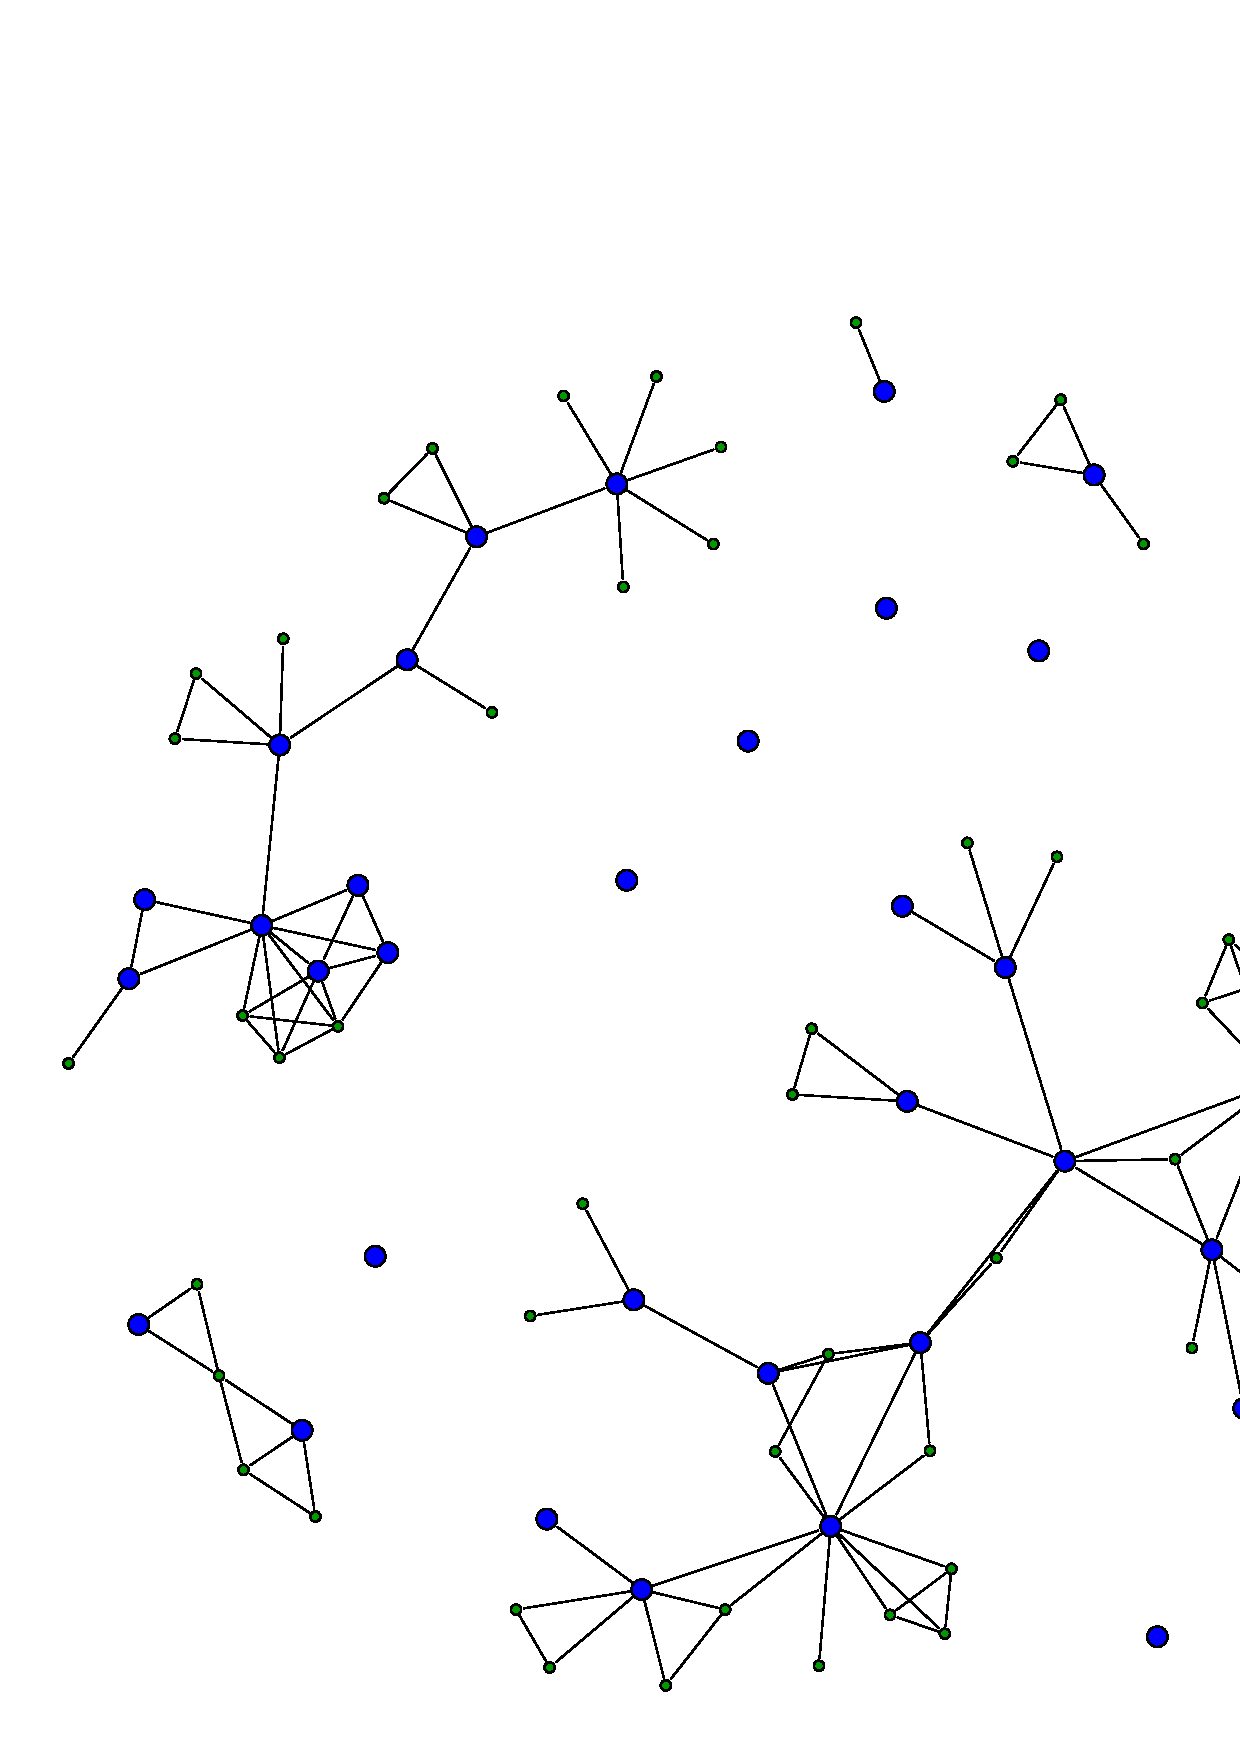
\includegraphics[width=.40\textwidth]{graph}
  \caption{Exemplo de grafo simples}
  \label{fig:humanbeta}
\end{figure}

Talvez você precise organizar a apresentação da informação na forma de
tabelas\index{Floats}. Um exemplo simples é a Tabela \ref{tab:amino_acidos}.

\begin{table}
\begin{center}
    \begin{tabular}{ccl}
    \rothead{Código} & \rothead{Abreviatura} & \rothead{Nome\\completo} \\ \hline
     \texttt{A}      & Ala                   & Alanina \\
     \texttt{C}      & Cys                   & Cisteína \\
     ...             & ...                   & ... \\
     \texttt{W}      & Trp                   & Tiptofano \\
     \texttt{Y}      & Tyr                   & Tirosina \\ \hline
    \end{tabular}
  \caption{Códigos, abreviaturas e nomes dos aminoácidos.}
  \label{tab:amino_acidos}
\end{center}
\end{table}

Há diversos estilos de tabela possíveis; A Tabela \ref{tab:ficha}, por
exemplo, mostra como construir uma tabela em forma de ficha larga que deve ser
impressa em modo paisagem. Um outro exemplo de tabela em modo paisagem, esta
distribuída em duas páginas, está no Apêndice \ref{ape:sequencias}.

% Aumenta o espaçamento entre as linhas da tabela (default: 0pt)
\setlength\extrarowheight{4pt}

\begin{sidewaystable}
\begin{tabular}{|M{0.265}|M{0.073}|M{0.084}|M{0.073}|M{0.073}|M{0.08}|M{0.082}|M{0.067}|}
  \hline
    \textbf{Experimento número:} & \multicolumn{2}{c|}{1} & \multicolumn{4}{c|}{\textbf{Data:}} & jan 2017
  \tabularnewline \hline
    \textbf{Título:} & \multicolumn{7}{c|}{Medições iniciais}
  \tabularnewline \hline
    \textbf{Tipo de experimento:} & \multicolumn{7}{c|}{Levantamento quantitativo}
  \tabularnewline \hline \hline
    \textbf{Locais}          & São Paulo & Rio de Janeiro & Porto Alegre & Recife & Manaus & Brasília & Rio Branco
  \tabularnewline \thickhline
    \textbf{Valores obtidos} & 0.2       & 0.3            & 0.2          & 0.7    & 0.5    & 0.1      & 0.4
  \tabularnewline \hline
\end{tabular}
\caption{Exemplo de tabela similar a uma ficha}
\label{tab:ficha}
\end{sidewaystable}

% Redefinindo para o valor default
\setlength\extrarowheight{0pt}

Pode também ser necessário apresentar trechos de código-fonte, o que pode
ser feito facilmente, como se vê na Figura \ref{fig:java}:\index{Floats}

% Foi utilizado o pacote listing para formatar código fonte
% http://ctan.org/tex-archive/macros/latex/contrib/listings/listings.pdf
% Veja no preambulo do arquivo tese-exemplo.tex os parâmetros de configuração.
\begin{figure}
  \index{Java}
  \centering
  \caption{Exemplo de laço em Java}
  \label{fig:java}
\begin{lstlisting}[language=Java, style=wider]
for(i = 0; i < 20; i++)
{
	// Comentário
	System.out.println("Mensagem...");
}
\end{lstlisting}
\end{figure}

\section{Modo Matemático}

O modo matemático do \LaTeX{} tem sintaxe própria, mas ela não é complicada
e há bastante documentação online a respeito. Um breve exemplo:

\begin{verbatim}
\begin{gather}
\label{eq:2grau}
    ax^2+bx+c=y \quad \forall x \in \mathbb{R}\\
\label{eq:bhaskara}
    y=0 \Leftrightarrow x=\frac{-b \pm \sqrt{\Delta}}{2a}
    \Leftrightarrow x \text{ é raiz da equação}\\
\label{eq:delta}
    \Delta\enspace(\mathit{delta}) = b^2-4ac
\end{gather}

As raízes de uma equação de segundo grau (Equação \ref{eq:2grau})
podem ser encontradas pela fórmula de Bháskara
(Equação \ref{eq:bhaskara}). O valor do discriminante $\Delta$
(Equação \ref{eq:delta}) determina se a equação tem zero, uma ou
duas raízes reais.
\end{verbatim}

Que resulta em:

\begin{gather}
\label{eq:2grau}
	ax^2+bx+c=y \quad \forall x \in \mathbb{R}\\
\label{eq:bhaskara}
    y=0 \Leftrightarrow x=\frac{-b \pm \sqrt{\Delta}}{2a}
    \Leftrightarrow x \text{ é raiz da equação}\\
\label{eq:delta}
    \Delta\enspace(\mathit{delta}) = b^2-4ac
\end{gather}

As raízes de uma equação de segundo grau (Equação \ref{eq:2grau})
podem ser encontradas pela fórmula de Bháskara
(Equação \ref{eq:bhaskara}). O valor do discriminante $\Delta$
(Equação \ref{eq:delta}) determina se a equação tem zero, uma ou
duas raízes reais.

\par

%% ------------------------------------------------------------------------- %%
\chapter{Conclus�es}
\label{cap:conclusoes}

Texto texto texto texto texto texto texto texto texto texto texto texto texto
texto texto texto texto texto texto texto texto texto texto texto texto texto
texto texto texto texto texto texto\footnote{Exemplo de refer�ncia para p�gina
Web: \url{www.vision.ime.usp.br/~jmena/stuff/tese-exemplo}}.

%------------------------------------------------------
\section{Considera��es Finais} 

Texto texto texto texto texto texto texto texto texto texto texto texto texto
texto texto texto texto texto texto texto texto texto texto texto texto texto
texto texto texto texto texto texto. 

%------------------------------------------------------
\section{Sugest�es para Pesquisas Futuras} 

Texto texto texto texto texto texto texto texto texto texto texto texto texto
texto texto texto texto texto texto texto texto texto texto texto texto texto
texto texto texto texto texto texto.

Finalmente, leia o trabalho de \citet{alon09:how} no qual apresenta-se
uma reflex�o sobre a utiliza��o da Lei de Pareto para tentar definir/escolher
problemas para as diferentes fases da vida acad�mica.  A dire��o dos novos
passos para a continuidade da vida acad�mica deveriam ser discutidos com seu
orientador.

\par


%%%%%%%%%%%%%%%%%%%%%%%%%%%%%%%% APÊNDICES %%%%%%%%%%%%%%%%%%%%%%%%%%%%%%%%%%%%%

% Aqui vão apêndices. O comando appendix reinicia a numeração de capítulos e
% passa a numerá-los com letras. Como os anteriores, ele não existe na classe
% "article".
\appendix

% Este formato está definido mais acima na seção "APARÊNCIA/FORMATAÇÃO"
\pagestyle{appendix}

% Os apêndices podem ser inseridos diretamente aqui ou "puxados" de outros
% arquivos
\chapter{Sequências}
\label{ape:sequencias}

Um exemplo de como o \LaTeX{} cria apêndices e uma referência para a Tabela
\ref{tab:numeros}, que é impressa em modo paisagem.

\singlespacing

% Reduz o espaçamento entre as colunas das tabelas (default: 1.0)
\renewcommand{\arraystretch}{0.85}

\captionsetup{margin=1.0cm}  % correção nas margens dos captions.
%--------------------------------------------------------------------------------------
\begin{landscape}
\begin{center}
\begin{longtable}{|c|c|c|c|c|c|c|c|c|c|c|c|c|}
\caption{Exemplo de tabela com valores numéricos.}\\
\hline
\emph{Limiar} &
\multicolumn{3}{c|}{MGWT} &
\multicolumn{3}{c|}{AMI} &
\multicolumn{3}{c|}{\emph{Spectrum} de Fourier} &
\multicolumn{3}{c|}{Características espectrais} \\
\cline{2-4} \cline{5-7} \cline{8-10} \cline{11-13} &
\emph{Sn} & \emph{Sp} & \emph{AC} &
\emph{Sn} & \emph{Sp} & \emph{AC} &
\emph{Sn} & \emph{Sp} & \emph{AC} &
\emph{Sn} & \emph{Sp} & \emph{AC} \\
\hline \hline
\endfirsthead
% Final do cabeçalho que aparece na primeira página; neste caso,
% igual ao das páginas seguintes, definido logo abaixo, exceto
% pelo comando caption; essa diferença impede que a lista de
% tabelas inclua uma referência para cada página da tabela

\caption[]{Exemplo de tabela com valores numéricos.}\\
\hline
\emph{Limiar} &
\multicolumn{3}{c|}{MGWT} &
\multicolumn{3}{c|}{AMI} &
\multicolumn{3}{c|}{\emph{Spectrum} de Fourier} &
\multicolumn{3}{c|}{Características espectrais} \\
\cline{2-4} \cline{5-7} \cline{8-10} \cline{11-13} &
\emph{Sn} & \emph{Sp} & \emph{AC} &
\emph{Sn} & \emph{Sp} & \emph{AC} &
\emph{Sn} & \emph{Sp} & \emph{AC} &
\emph{Sn} & \emph{Sp} & \emph{AC} \\
\hline \hline
\endhead % Final do cabeçalho que aparece em todas as páginas

\hline
\multicolumn{13}{|r|}{Continua...}\\
\hline
\endfoot % Final do rodapé que aparece em todas as páginas exceto a última

\hline
\endlastfoot % Final do rodapé da última página (neste caso, apenas uma linha)
\label{tab:numeros} % O label não deve ficar em um cabeçalho que se repete!
 1 & 1.00 & 0.16 & 0.08 & 1.00 & 0.16 & 0.08 & 1.00 & 0.16 & 0.08 & 1.00 & 0.16 & 0.08 \\
 2 & 1.00 & 0.16 & 0.09 & 1.00 & 0.16 & 0.09 & 1.00 & 0.16 & 0.09 & 1.00 & 0.16 & 0.09 \\
 3 & 1.00 & 0.16 & 0.10 & 1.00 & 0.16 & 0.10 & 1.00 & 0.16 & 0.10 & 1.00 & 0.16 & 0.10 \\
 4 & 1.00 & 0.16 & 0.10 & 1.00 & 0.16 & 0.10 & 1.00 & 0.16 & 0.10 & 1.00 & 0.16 & 0.10 \\
 5 & 1.00 & 0.16 & 0.11 & 1.00 & 0.16 & 0.11 & 1.00 & 0.16 & 0.11 & 1.00 & 0.16 & 0.11 \\
 6 & 1.00 & 0.16 & 0.12 & 1.00 & 0.16 & 0.12 & 1.00 & 0.16 & 0.12 & 1.00 & 0.16 & 0.12 \\
 7 & 1.00 & 0.17 & 0.12 & 1.00 & 0.17 & 0.12 & 1.00 & 0.17 & 0.12 & 1.00 & 0.17 & 0.13 \\
 8 & 1.00 & 0.17 & 0.13 & 1.00 & 0.17 & 0.13 & 1.00 & 0.17 & 0.13 & 1.00 & 0.17 & 0.13 \\
 9 & 1.00 & 0.17 & 0.14 & 1.00 & 0.17 & 0.14 & 1.00 & 0.17 & 0.14 & 1.00 & 0.17 & 0.14 \\
10 & 1.00 & 0.17 & 0.15 & 1.00 & 0.17 & 0.15 & 1.00 & 0.17 & 0.15 & 1.00 & 0.17 & 0.15 \\
11 & 1.00 & 0.17 & 0.15 & 1.00 & 0.17 & 0.15 & 1.00 & 0.17 & 0.15 & 1.00 & 0.17 & 0.15 \\
12 & 1.00 & 0.18 & 0.16 & 1.00 & 0.18 & 0.16 & 1.00 & 0.18 & 0.16 & 1.00 & 0.18 & 0.16 \\
13 & 1.00 & 0.18 & 0.17 & 1.00 & 0.18 & 0.17 & 1.00 & 0.18 & 0.17 & 1.00 & 0.18 & 0.17 \\
14 & 1.00 & 0.18 & 0.17 & 1.00 & 0.18 & 0.17 & 1.00 & 0.18 & 0.17 & 1.00 & 0.18 & 0.17 \\
15 & 1.00 & 0.18 & 0.18 & 1.00 & 0.18 & 0.18 & 1.00 & 0.18 & 0.18 & 1.00 & 0.18 & 0.18 \\
16 & 1.00 & 0.18 & 0.19 & 1.00 & 0.18 & 0.19 & 1.00 & 0.18 & 0.19 & 1.00 & 0.18 & 0.19 \\
17 & 1.00 & 0.19 & 0.19 & 1.00 & 0.19 & 0.19 & 1.00 & 0.19 & 0.19 & 1.00 & 0.19 & 0.19 \\
18 & 1.00 & 0.19 & 0.20 & 1.00 & 0.19 & 0.20 & 1.00 & 0.19 & 0.20 & 1.00 & 0.19 & 0.20 \\
19 & 1.00 & 0.19 & 0.21 & 1.00 & 0.19 & 0.21 & 1.00 & 0.19 & 0.21 & 1.00 & 0.19 & 0.21 \\
20 & 1.00 & 0.19 & 0.22 & 1.00 & 0.19 & 0.22 & 1.00 & 0.19 & 0.22 & 1.00 & 0.19 & 0.22 \\
21 & 1.00 & 0.19 & 0.22 & 1.00 & 0.19 & 0.22 & 1.00 & 0.19 & 0.22 & 1.00 & 0.19 & 0.22 \\
22 & 1.00 & 0.19 & 0.22 & 1.00 & 0.19 & 0.22 & 1.00 & 0.19 & 0.22 & 1.00 & 0.19 & 0.22 \\
23 & 1.00 & 0.19 & 0.22 & 1.00 & 0.19 & 0.22 & 1.00 & 0.19 & 0.22 & 1.00 & 0.19 & 0.22 \\
24 & 1.00 & 0.19 & 0.22 & 1.00 & 0.19 & 0.22 & 1.00 & 0.19 & 0.22 & 1.00 & 0.19 & 0.22 \\
25 & 1.00 & 0.19 & 0.22 & 1.00 & 0.19 & 0.22 & 1.00 & 0.19 & 0.22 & 1.00 & 0.19 & 0.22 \\
26 & 1.00 & 0.19 & 0.22 & 1.00 & 0.19 & 0.22 & 1.00 & 0.19 & 0.22 & 1.00 & 0.19 & 0.22 \\
27 & 1.00 & 0.19 & 0.22 & 1.00 & 0.19 & 0.22 & 1.00 & 0.19 & 0.22 & 1.00 & 0.19 & 0.22 \\
28 & 1.00 & 0.19 & 0.22 & 1.00 & 0.19 & 0.22 & 1.00 & 0.19 & 0.22 & 1.00 & 0.19 & 0.22 \\
29 & 1.00 & 0.19 & 0.22 & 1.00 & 0.19 & 0.22 & 1.00 & 0.19 & 0.22 & 1.00 & 0.19 & 0.22 \\
30 & 1.00 & 0.19 & 0.22 & 1.00 & 0.19 & 0.22 & 1.00 & 0.19 & 0.22 & 1.00 & 0.19 & 0.22 \\
31 & 1.00 & 0.19 & 0.22 & 1.00 & 0.19 & 0.22 & 1.00 & 0.19 & 0.22 & 1.00 & 0.19 & 0.22 \\
32 & 1.00 & 0.19 & 0.22 & 1.00 & 0.19 & 0.22 & 1.00 & 0.19 & 0.22 & 1.00 & 0.19 & 0.22 \\
33 & 1.00 & 0.19 & 0.22 & 1.00 & 0.19 & 0.22 & 1.00 & 0.19 & 0.22 & 1.00 & 0.19 & 0.22 \\
34 & 1.00 & 0.19 & 0.22 & 1.00 & 0.19 & 0.22 & 1.00 & 0.19 & 0.22 & 1.00 & 0.19 & 0.22 \\
35 & 1.00 & 0.19 & 0.22 & 1.00 & 0.19 & 0.22 & 1.00 & 0.19 & 0.22 & 1.00 & 0.19 & 0.22 \\
36 & 1.00 & 0.19 & 0.22 & 1.00 & 0.19 & 0.22 & 1.00 & 0.19 & 0.22 & 1.00 & 0.19 & 0.22 \\
37 & 1.00 & 0.19 & 0.22 & 1.00 & 0.19 & 0.22 & 1.00 & 0.19 & 0.22 & 1.00 & 0.19 & 0.22 \\
38 & 1.00 & 0.19 & 0.22 & 1.00 & 0.19 & 0.22 & 1.00 & 0.19 & 0.22 & 1.00 & 0.19 & 0.22 \\
39 & 1.00 & 0.19 & 0.22 & 1.00 & 0.19 & 0.22 & 1.00 & 0.19 & 0.22 & 1.00 & 0.19 & 0.22 \\
40 & 1.00 & 0.19 & 0.22 & 1.00 & 0.19 & 0.22 & 1.00 & 0.19 & 0.22 & 1.00 & 0.19 & 0.22 \\
41 & 1.00 & 0.19 & 0.22 & 1.00 & 0.19 & 0.22 & 1.00 & 0.19 & 0.22 & 1.00 & 0.19 & 0.22 \\
42 & 1.00 & 0.19 & 0.22 & 1.00 & 0.19 & 0.22 & 1.00 & 0.19 & 0.22 & 1.00 & 0.19 & 0.22 \\
43 & 1.00 & 0.19 & 0.22 & 1.00 & 0.19 & 0.22 & 1.00 & 0.19 & 0.22 & 1.00 & 0.19 & 0.22 \\
44 & 1.00 & 0.19 & 0.22 & 1.00 & 0.19 & 0.22 & 1.00 & 0.19 & 0.22 & 1.00 & 0.19 & 0.22 \\
45 & 1.00 & 0.19 & 0.22 & 1.00 & 0.19 & 0.22 & 1.00 & 0.19 & 0.22 & 1.00 & 0.19 & 0.22 \\
46 & 1.00 & 0.19 & 0.22 & 1.00 & 0.19 & 0.22 & 1.00 & 0.19 & 0.22 & 1.00 & 0.19 & 0.22 \\
47 & 1.00 & 0.19 & 0.22 & 1.00 & 0.19 & 0.22 & 1.00 & 0.19 & 0.22 & 1.00 & 0.19 & 0.22 \\
48 & 1.00 & 0.19 & 0.22 & 1.00 & 0.19 & 0.22 & 1.00 & 0.19 & 0.22 & 1.00 & 0.19 & 0.22 \\
49 & 1.00 & 0.19 & 0.22 & 1.00 & 0.19 & 0.22 & 1.00 & 0.19 & 0.22 & 1.00 & 0.19 & 0.22 \\
\end{longtable}
\end{center}
\end{landscape}

% É uma boa ideia redefinir os valores default
\renewcommand{\arraystretch}{1.0}

\par

%%%%%%%%%%%%%%%%%%%%%%%%%%%%%% SEÇÕES FINAIS %%%%%%%%%%%%%%%%%%%%%%%%%%%%%%%%%%%

% Aqui vão a bibliografia, índice remissivo e outras seções similares.
% O comando backmatter desabilita a numeração de capítulos e também não existe
% na classe "article".
\backmatter

% Este formato está definido mais acima na seção "APARÊNCIA/FORMATAÇÃO"
\pagestyle{frontback}

\singlespacing   % espaçamento simples

% A bibliografia é obrigatória

%%%%%%%%% Bibliografia com natbib (preterido): %%%%%%%%%
%\bibliographystyle{alpha-ime}% citação bibliográfica alpha
%\bibliographystyle{plainnat-ime} % citação bibliográfica textual
%\bibliography{bibliografia}  % associado ao arquivo: 'bibliografia.bib'

%%%%%%%% Bibliografia com biblatex (preferido): %%%%%%%%

\printbibliography[
  title=Bibliografia\label{bibliografia},
  % Inclui a bibliografia no sumário; comente se estiver usando "article"
  heading=bibintoc,
]

% imprime o índice remissivo no documento (opcional)
\printindex

\end{document}
